\documentclass[final,c]{beamer}
\mode<presentation>
{
  \usetheme{PaloAlto}
  \usecolortheme{default}
  \setbeamercovered{transparent}
}
\setbeamertemplate{nabigation symbols}{}

\usepackage{luatexja}
\usepackage{luatexja-otf}
\usepackage[match]{luatexja-fontspec}
\usepackage[hiragino-pron,deluxe,expert]{luatexja-preset}

\usepackage{times}
\usepackage[T1]{fontenc}
\usepackage{lmodern}
\usepackage{ascmac}
\usepackage{amssymb,amsmath}
\usepackage{txfonts}
\usepackage{proof}
\usepackage{graphicx}
\usepackage{multimedia}
\usepackage{filecontents}
\usepackage{bxdpx-beamer}
\usepackage{listings}
\usepackage{tikz} % To generate the plot from csv
\usepackage{pgfplots}

%\renewcommand{\ttdefault}{lmtl}
\newcommand{\jpy}{{{\ooalign{Y\crcr\hss=\hss}}}}
\newcommand{\combination}[2]{{}_{#1}C_{#2}}
\newcommand{\lstref}[1]{Listing \ref{#1}}

\lstset{language=python,%
   basicstyle={\ttfamily\tiny},%
%   lineskip=-0.5zw,%
   commentstyle=\textit,%
   classoffset=1,%
   keywordstyle=\bfseries,%
   breaklines=true,
   frame=lines,%
   framesep=5pt,%
   showstringspaces=false,%
   numbers=left,%
   numbersep=3pt,%
   stepnumber=1,%
   numberstyle={\ttfamily\tiny},%
%   numberstyle={\tiny},%
   numberblanklines=true,
%   morekeywords={def, end, while, if, for, in, else, then, return}%
}%

\pgfplotsset{
   compat=newest,
%   width=10cm,
   tick label style={font=\footnotesize},
   label style={font=\footnotesize},
   legend style={font=\footnotesize},
   every axis/.append style={very thick},
}%

\title[elementaryCS-2nd]{コンピュータサイエンス入門第二}
\date[4th quarter]{4th quarter}
\author[Naoyuki Nagatou]{永藤 直行}
\institute[TITECH]{東京工業大学}

\subject{Lecture}

% Delete this, if you do not want the table of contents to pop up at
% the beginning of each subsection:
%\AtBeginSubsection[]
%{
%  \begin{frame}<beamer>{Outline}
%    \tableofcontents[currentsection,currentsubsection]
%  \end{frame}
%}
\AtBeginSection{
  \begin{frame}
\frametitle{Outline}
\scriptsize
\tableofcontents[currentsection]
  \end{frame}
}
\AtBeginPart{\frame{\partpage}}

% If you wish to uncover everything in a step-wise fashion, uncomment
% the following command: 
%\beamerdefaultoverlayspecification{<+->}

\begin{document}
\frame{\titlepage}
%
%%% PROLOGUE
%
\part{Prologue}
\frame{
  \frametitle{Prologue}
  \tableofcontents[part=1]
}
%
%%% REFERENCE
%
\section{教科書,参考文献}
%\begin{frame}
%\frametitle{教科書}
%  \begin{itemize}
%\item CS 第 1 とおなじ
%\item 教科書: 渡辺治 著,コンピュータサイエンス\textendash 計算を通して世界を観る, 丸善出版 (2015)
%\item 教科書のサイト: \href{http://www.is.titech.ac.jp/~watanabe/csbook/}{\beamerbutton{http://www.is.titech.ac.jp/$\sim$watanabe/csbook/}} 
%\item 4b(CS2) クラスのサイト: \href{https://sites.google.com/a/presystems.xyz/sample/home/elementary-computer-science}{\beamerbutton{https://sites.google.com/a/presystems.xyz/sample/home/elementary-computer-science}} 
%  \end{itemize}
%\centering
%
\includegraphics[scale=.25]{./Figure/TextBook.jpg}
%\end{frame}
\begin{frame}[shrink]
\frametitle{参考図書}
  \begin{itemize}
\item \href{https://www.mheducation.com/highered/product/discrete-mathematics-applications-rosen/M0073383090.html}{\beamerbutton{Discrete Mathematics and its Applications}}
\item Structure and Interpretation of Computer Programs \href{http://web.mit.edu/alexmv/6.037/sicp.pdf}{\beamerbutton{http://web.mit.edu/alexmv/6.037/sicp.pdf}} 
\item 計算機プログラムの構造と解釈 (日本語訳)\\ \href{http://sicp.iijlab.net/fulltext/xcont.html}{\beamerbutton{http://sicp.iijlab.net/fulltext/xcont.html}} 
  \end{itemize}
  \begin{columns}[c]
    \begin{column}{0.5\textwidth}
\centering
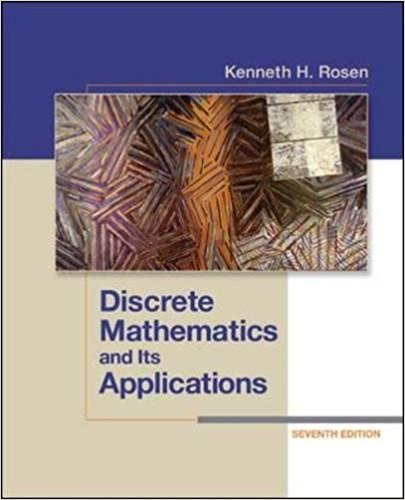
\includegraphics[scale=.25]{./Figure/Discrete_Mathematics_And_its_Applications.jpg}
    \end{column}
    \begin{column}{0.45\textwidth}
\centering
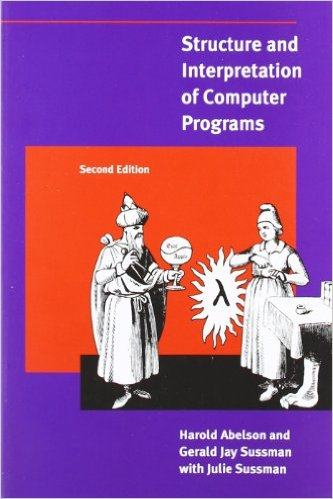
\includegraphics[scale=.25]{./Figure/SICP.jpg}
    \end{column}
  \end{columns}
\end{frame}
%
%%% GOAL
%
\section{講義概要}
\begin{frame}
\frametitle{講義概要}
  \begin{itemize}
\item 利用する教室,演習室は OCW-i を参照
\item 講義スケジュール:
    \begin{enumerate}
\item 再帰
\item よいアルゴリズム,わるいアルゴリズム,ふつうのアルゴリズム
%\item 大きい数と小さい数の計算 (実数の計算)
    \end{enumerate}
  \end{itemize}
  \begin{block}{目標}
計算でものを表すとき便利な道具と注意すべきことを会得すること
  \end{block}
\end{frame}
%
%%% EVALUATION
%
\section{評価基準}
\begin{frame}
\frametitle{評価基準}
  \begin{itemize}
\item 講義は全 6 回と試験 1 回
\item 課題: 3 回 (計 70 点)
\item 課題提出: 
    \begin{itemize}
\item 講義時間中に課題を出します
\item 提出方法はその都度指定します
    \end{itemize}
\item 期末試験 (30 点)
  \end{itemize}
\end{frame}

%
%%% 再帰
%
\part{再帰}
\frame{
  \frametitle{再帰}
\scriptsize
  \tableofcontents[part=2]
}
\section{再帰 (Recursion)}
\subsection{再帰への導入}
\begin{frame}[fragile]
\frametitle{再帰への導入}
  \begin{itemize}
\item 対象を簡潔に明示的に表す方法
\item たとえば下の絵,ひとつ絵を書いてその中央にその絵を書ている(Droste 効果)
\item 対象を定義するときに既にわかっている部分を参照して定義するということ

%\item 関数を合成することで別の関数を定義できる
%\item 複雑な計算を定義する時にはより単純な部分問題に分割して,単純な計算を合成する
  \end{itemize}
  \begin{center}
\includegraphics[scale=0.4]{../Figure/Rosen_picture.jpg}
  \end{center}
\end{frame}
\begin{frame}[fragile,shrink]
\frametitle{数列の再帰的定義}
  \begin{itemize}
\item 数列 \(a_n=\frac{n(n+1)}{2},\ n\leq 1\)
\item Baseic step (初項) を 1
\item Recursive step (n 項) を \(a_n=n+a_{n-1}\) と定義できる
\item \(n\) 項を決めるのに \(n-1\) 項から決める
\item まだ決まっていない最小の項を既に知っている項から決定する
  \end{itemize}
  \begin{columns}
    \begin{column}[t]{0.4\textwidth}
      \begin{center}
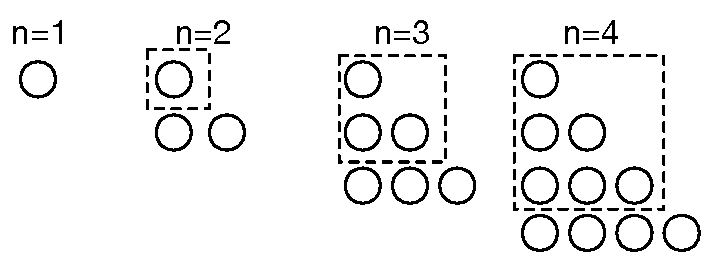
\includegraphics[scale=0.4]{./Figure/elementaryCS-figTriangular.pdf}
      \end{center}
    \end{column}
    \begin{column}[t]{0.4\textwidth}
      \begin{center}
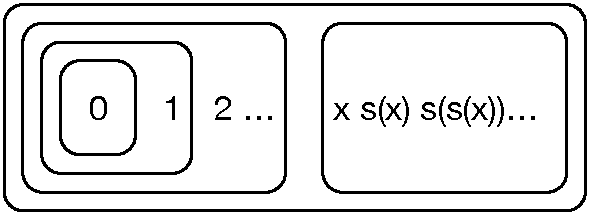
\includegraphics[scale=0.4]{./Figure/elementaryCS-2nd-figRecursion.pdf}
      \end{center}
    \end{column}
  \end{columns}
\end{frame}
\subsection{再帰 (Recursion)}
\begin{frame}[fragile]
\frametitle{再帰的定義の原理}
  \begin{itemize}
\item 関数 $f$ の定義に $x$ より小さい要素についての評価を利用して定義することを原始再帰 (primitive recursion) と呼ぶ
\item $x$ より小さい値についての評価はいつも同じ値と仮定
\item 定義できた最大の $x$ のつぎの値について定義するというのを繰り返すと全体について定義できる (\(\delta\)-近似)
  \end{itemize}
  \begin{theorem}[再帰の原理]
\scriptsize
順序数 (自然数は順序数) \(x\) として,
    \begin{center}
\(f(x)=G(f\upharpoonright x)\)
    \end{center}
ここで,\(f\upharpoonright x\) は \(f\) を \(x\) より小さい数に制限したもの, $G$ は計算のしかたを表したもの
  \end{theorem}
  \begin{center}
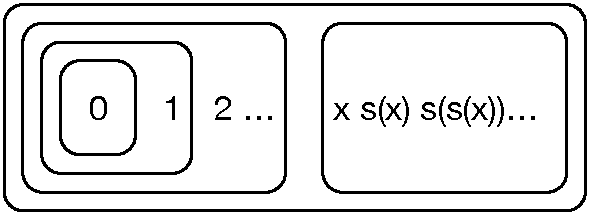
\includegraphics[scale=0.5]{./Figure/elementaryCS-2nd-figRecursion.pdf}
  \end{center}
\end{frame}
\subsection{再帰的定義}
\begin{frame}[fragile,shrink]
\frametitle{関数の再帰的定義}
\framesubtitle{加算,乗算の再帰的定義}
   \begin{itemize}
%\item Basic step と recursive step をそれぞれ定義
\item G に相当するのが \(\operatorname{succ}\)
\item Basic step に近づけるように recursive step を定義
     \begin{itemize}
\item \(a+\operatorname{succ}(b)=\operatorname{succ}(a+b)\)
     \end{itemize}
  \end{itemize}
\vspace{-1em}
  \begin{center}
  \begin{math}
    \begin{array}{lll}
\mbox{Basic step:}& a+0 & \mbox{if }b=0 \\
\mbox{Recusive step:}& \operatorname{succ}(a+b) & \mbox{otherwise}
    \end{array}
  \end{math}  
  \end{center}
\vspace{-2em}
  \begin{columns}
    \begin{column}[t]{0.4\textwidth}
      \begin{lstlisting}[caption={加算},label=add-rec]
# Recursive definition
import os
import time

def succ (x):
  return(x+1)
def pred (x):
  return(x-1)
def add (a,b):
  if (b==0):
    return(a)
  else:
    return(succ(add(a,pred(b))))
      \end{lstlisting}
    \end{column}
    \begin{column}[t]{0.55\textwidth}
      \begin{lstlisting}[firstnumber=15,caption={乗算},label=mult-rec]
# Multiplication
#
def mult (a,b):
  if (b==0):
    return(0)
  else:
    return(add(add(0,a),mult(a,pred(b))))
      \end{lstlisting}
    \end{column}
  \end{columns}
\end{frame}
\begin{frame}[fragile,shrink]
\frametitle{再帰的定義の例 1}
\framesubtitle{Factorial}
  \begin{itemize}
\item \(n!=n\cdot(n-1)\cdot(n-2)\cdots 3\cdot 2\cdot 1\)
\item \(n!\) を決めるのに \((n-1)!\) の値をつかう
\item G に相当するのが \(n\cdot(n-1)!\) ということ
\item まだ決まっていない最小の値は決まっている値で最大の値のつぎになる
  \end{itemize}
  \begin{columns}[c]
    \begin{column}{0.5\textwidth}
      \begin{lstlisting}[caption={階乗},label=fact-rec]
def fact (n):
  if (n == 1):
    return(1)
  else:
    return(n*(fact(n-1)))
      \end{lstlisting}
    \end{column}
    \begin{column}{0.45\textwidth}
      \begin{example}[\(4!\)]
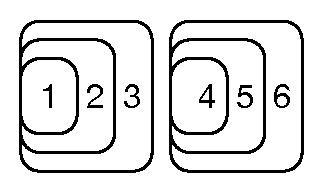
\includegraphics[scale=0.5]{./Figure/elementaryCS-2nd-figFact.eps}
      \end{example}
    \end{column}
  \end{columns}
\end{frame}
\begin{frame}[fragile]
\frametitle{フィボナッチ数}
  \begin{itemize}
\item 突然ですが次の問題を考えてみてください
  \end{itemize}
  \begin{block}{うさぎとフィボナッチ数}
    \begin{itemize}
\item $n$ ヶ月後のうさぎのつがいは何組?
\item 最初一組のつがいだけ
\item 2 ヶ月経つと メス 1 匹を生んでそのつがいが 1 組増える
\item うさぎは決して死なない
    \end{itemize}
  \end{block}
  \begin{center}
    \begin{tabular}{ccccc}
月&生後 0 ヶ月&生後 2 ヶ月以下&合計\\
\hline
1&0&1&1\\
2&0&1&1\\
3&1&1&2\\
4&1&2&3\\
    \end{tabular}
  \end{center}
\end{frame}
\begin{frame}[fragile]
\frametitle{再帰的定義の例 2}
  \begin{itemize}
\item フィボナッチ数\\
    \begin{tabular}{c|c|c|c|c|c}
0&1&2&3&4&5$\cdots$\\
\hline
1&1&2&3&5&8$\cdots$
    \end{tabular}
\item \({\mathop{\mathrm{fib}}}(S(n))\) を決めるのに \({\mathop{\mathrm{fib}}}(n)\) と \({\mathop{\mathrm{fib}}}(n-1)\) を使う
\item G に相当するのが \(n\) と \(n-1\) のフィボナッチ数を足し合わせるということ
  \end{itemize}
  \begin{columns}[c]
    \begin{column}{0.5\textwidth}
      \begin{lstlisting}[caption={フィボナッチ数},label=fib-rec]
def fib (n):
  if (n==0):
    return(0)
  else:
    if (n==1):
      return(1)
    else:
      return(fib(n-1)+fib(n-2))
      \end{lstlisting}
    \end{column}
    \begin{column}{0.45\textwidth}
      \begin{example}[fib\((5)\)]
        \begin{center}
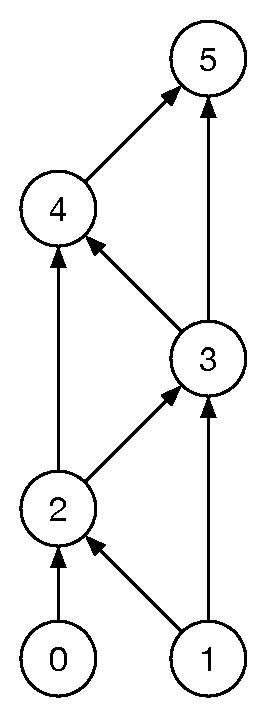
\includegraphics[scale=0.3]{./Figure/elementaryCS-2nd-figFib.eps}
        \end{center}
      \end{example}
    \end{column}
  \end{columns}
\end{frame}
\begin{frame}[fragile]
\frametitle{集合の再帰的定義}
  \begin{itemize}
\item Basic step: 集合の初期要素を定義
\item Recursive step: 既にわかっている要素から新しい要素を定義する規則
  \end{itemize}
%  \begin{example}[3 の倍数]
%    \begin{itemize}
%\item Basic step: 3 は集合の要素
%\item Recursive step: 集合の要素 \(x,y\) として \(x+y\) も要素
%\item E.g. : \(\{3,\ 3+3=6,\ 3+6=9,\ 6+6=12,\cdots\}\)
%    \end{itemize}
%  \end{example}
  \begin{example}[文字列の集合\(\Sigma*\)]
    \begin{itemize}
\item Basic step: \(\epsilon\in\Sigma\) (空列 \(\epsilon\) も \(\Sigma\) に含まれる)
\item Recursive step: \(a\in\Sigma,w\in\Sigma*\) ならば \(aw\in\Sigma*\)
\item E.g.: \(\{\epsilon,\ a,\ aa,\ aaa,\cdots\}\)
    \end{itemize}
  \end{example}
\end{frame}
\subsection{木構造}
\begin{frame}[fragile]
\frametitle{Tree (木構造)}
  \begin{itemize}
\item 数以外も
\item Basic step: vertex $r$ は tree
\item Recursive step: \(T_1,T_2,\cdots,T_n\) それぞれ root を \(r_1,r_2,\cdots,r_n\) とする tree として,
\(r\) から \(r_1,r_2,\cdots,r_n\) への edge 追加したものもまた tree である
  \end{itemize}
  \begin{center}
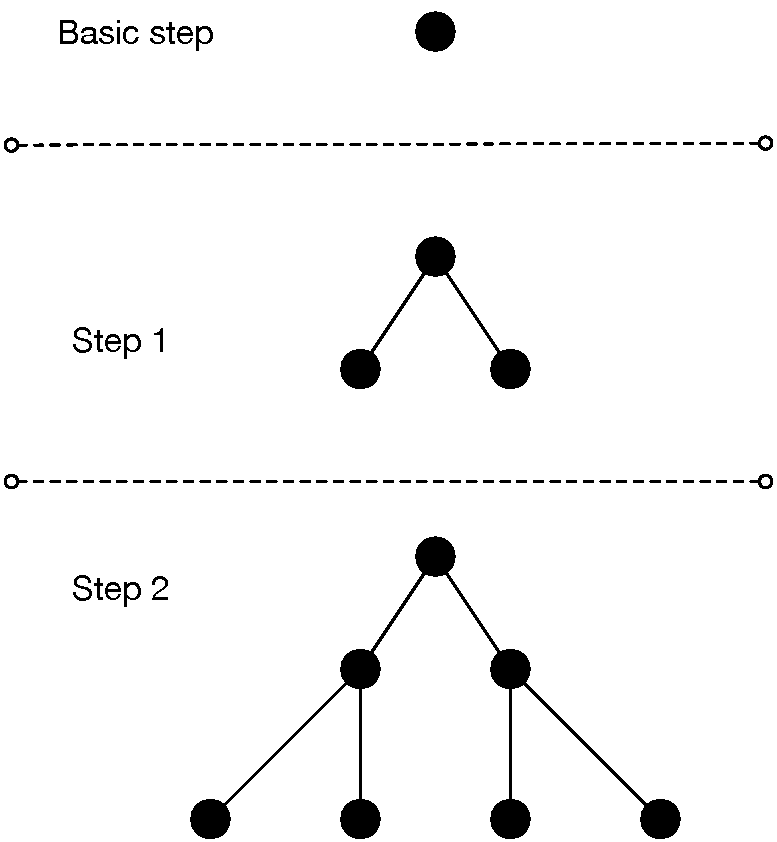
\includegraphics[scale=0.3]{./Figure/elementaryCS-tree.pdf}
  \end{center}
\end{frame}
\begin{frame}[fragile]
\frametitle{再帰は強力な道具}
  \begin{itemize}
\item 最初の元から順番に対象を構成
\item 対象が順番に並べられるなら
\item 問題を解く時も,最も小さい問題の解から順番に全体の解を構成することができる
\item (いつもではないけど)
  \end{itemize}
\end{frame}
\begin{frame}[fragile]
\frametitle{宿題 1}
  \begin{itemize}
\item 自然数上の四則演算を再帰で定義し直してみてください
\item フィボナッチ数を求める再帰的な計算を繰り返しに直してみてください
\item 先の文字列の集合を参考に文字列の長さを求める関数を再帰的に定義せよ.
    \begin{itemize}
\item Hint: Basic step を空列は長さ 0 として,recursive step は一文字短い文字列より 1 長い
\item Python では str[1:] とすると文字列の 2 番目以降の文字列を得ることができる
\item 空列は not str  あるいは len(str) で判定
    \end{itemize}
  \end{itemize}
\end{frame}
\section{プログラムとしての再帰}
\subsection{引数の有効範囲 (Scope)}
\begin{frame}[fragile,shrink]
\frametitle{仮引数と実引数}
\scriptsize
  \begin{itemize}
\item CS 第 1 では手続きに名前をつけて抽象化することをみた
\item 関数は 0 個以上の仮引数というものをもつ
    \begin{itemize}
\scriptsize
\item 下の例では {\tt n, eps} などが仮引数
    \end{itemize}
%\item 複数の関数が同じ名前の仮引数を持っていても良い
\item 仮引数は関数の本体で有効である
\item 関数を呼び出したときの値に束縛 (bind) されて,関数の本体では呼び出し時の値に置き換えられる
\item 呼び出し時の値を実引数という
\item 一般に変数は有効範囲 (scope) が決まっている
\item 仮引数は関数本体が有効範囲である
  \end{itemize}
\vspace{-3em}
  \begin{columns}[t]
    \begin{column}{0.5\textwidth}
      \begin{lstlisting}[caption={Newton 法},label=newton-rec]
### Newton's method 
def sqrt_iter (guess,n,eps,previous):
  def is_enough (guess,eps,previous):
    return(abs(previous-guess)<(2*eps))
  def improve (guess,n):
    return((guess+(n/guess))/2.0)
  if is_enough(guess,eps,previous):
     return(guess)
  else:
     return(sqrt_iter(improve(guess,n),n,eps,guess))
def sqroot1 (n,eps):
  return(sqrt_iter(1.0,n,(2*eps),0.0))
      \end{lstlisting}
    \end{column}
    \begin{column}{0.45\textwidth}
      \begin{lstlisting}[caption={Newton 法},firstnumber=13,label=newton-is_enough-rec]
def sqroot (n):
  ### Machine epsilon
  def eps_m ():
    epsilon, old, prod = 1.0, 0.0, 0.0
    cnt=0
    while (prod!=1.0):
      old = epsilon
      cnt=cnt+1
      epsilon=epsilon/2.0
      prod=epsilon+1.0
    return(old)
  return(sqroot1(n,eps_m()))
      \end{lstlisting}
    \end{column}
  \end{columns}
\end{frame}
\subsection{再帰プログラム}
\begin{frame}[fragile]
\frametitle{プログラムとしての再帰}
  \begin{itemize}
\item プログラムでも関数を定義するときに自身をもちいることができる
\item 下のプログラムを実行してみるので引数の値に注意して見ていてください
\item 関数は定義しただけでは実行されず,呼び出したときはじめて活性化され,仮引数が束縛される
    \begin{itemize}
\item {\tt n} は 3,2,1 と束縛される
    \end{itemize}
  \end{itemize}
  \begin{columns}[c]
    \begin{column}{0.6\textwidth}
      \begin{lstlisting}[caption={階乗 (引数表示版)},label=fact-with-puts]
# Factorial
def fact (n):
  if (n == 1):
    return(1)
  else:
    return(n*(fact(n-1)))
      \end{lstlisting}
    \end{column}
    \begin{column}{0.35\textwidth}
      \begin{center}
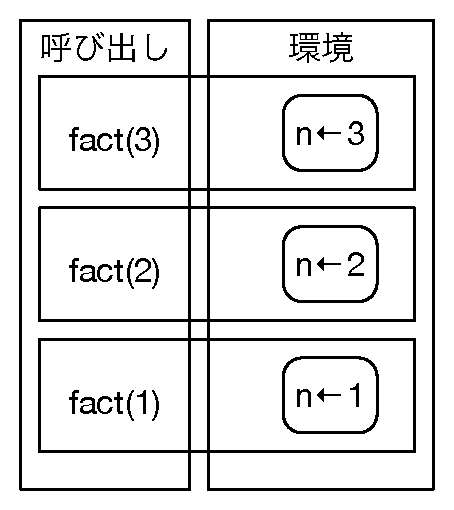
\includegraphics[scale=0.3]{./Figure/elementaryCS-2nd-figStack.eps}
      \end{center}
    \end{column}
  \end{columns}
\end{frame}
\begin{frame}[fragile]
\frametitle{関数の評価と生成プロセス}
  \begin{itembox}{fact(4) の生成プロセス}
    \begin{verbatim}
  fact(4)
=>(4 * fact(3))
=>(4 * (3 * fact(2)))
=>(4 * (3 * (2 * fact(1))))
=>(4 * (3 * (2 * 1)))
=>(4 * (3 * 2 ))
=>(4 * 6)
=>24
    \end{verbatim}
  \end{itembox}
\end{frame}
%\subsection{分割統治法 (Devide and Conquer)}
%\begin{frame}[fragile]
%\frametitle{分割統治法 (Devide and Conquer)}
%  \begin{itemize}
%\item 分割統治法とは複雑な問題をより簡単な部分問題に分割し,部分問題の解から合成して全体の解を求めるという方法
%\item 分割統治法は再帰プログラムとしてあらわせる
%  \end{itemize}
%  \begin{example}[組合せ (Comination)の部分問題への分割]
%    \begin{itemize}
%\item \(\combination{n}{r}=0\) 
%      \begin{itemize}
%\item \(n,r,n-r<0\) のときの数
%      \end{itemize}
%\item \(\combination{n}{0}=1\) 
%      \begin{itemize}
%\item $n$ 個から $0$ 個取り出したときの数
%      \end{itemize}
%\item \(\combination{n}{r}=\combination{n-1}{r}+\combination{n-1}{r-1}\) 
%      \begin{itemize}
%\item $n$ 個から $1$ 個を除外して残り \(r-1\) を選ぶ場合
%\item $n$ 個から $1$ 個取り出して残り \(r-1\) を選ぶ場合
%      \end{itemize}
%\item \(n,r\) が小さくなっているだけで同じ問題
%    \end{itemize}
%  \end{example}
%\end{frame}
%\begin{frame}[fragile]
%\frametitle{\(\combination{n}{r}\) の定義}
%%  \begin{itemize}
%%\item 以下の定義とプログラムを得る
%%  \end{itemize}
%  \begin{definition}[\(\combination{n}{r}\)]
%\[\combination{n}{r}=\left\{
%      \begin{array}{ll}
%0 & \mbox{if } n,r,n-r<0\\
%1 & \mbox{if } r=0\\
%\combination{n-1}{r-1}+\combination{n-1}{r} & \mbox{otherwise}\\
%      \end{array}
%\right.\]
%  \end{definition}
%  \begin{lstlisting}[caption={組み合わせの数},label=comb]
%# Combination n, r
%def comb (n,r)
%  if ((n-r)<0||n<0||r<0) then
%    return 0
%  else
%    if (r==0) then
%      return 1
%    else
%      return (comb(n-1,r)+comb(n-1,r-1))
%    end
%  end
%end
%### Test Harness
%x = gets().to_i
%y = gets().to_i
%puts "C(n,r)="
%puts(comb(x,y))
%  \end{lstlisting}
%\end{frame}
\subsection{帰納法 (Induction)}
\begin{frame}[fragile]
\frametitle{帰納法の原理}
  \begin{itemize}
\item 帰納法は再帰的に定義されたものの性質を証明するテクニック
\item 再帰的アルゴリズムの正当性を証明するのにも使える
\item 下に帰納法の原理をあげておきます
\item \(\operatorname{succ}(y)\) は $y$ のつぎの数という意味です (CS 入門第一の\(+1\) に相当)
\item 証明したいことがらを \(\phi\) とします
\item 原理の前提条件を充たすことを示します \(\phi(0)\wedge(\phi(n)\Rightarrow\phi(\operatorname{succ}(n)))\)
  \end{itemize}
  \begin{block}{帰納法の原理}
集合 \(X=\{n\colon \phi(n)\}\) について,もし \(0\in X\) かつ \(\forall y\in X\colon \operatorname{succ}(y)\in X\) であるなら,$X$ はすべての自然数を含む
  \end{block}
\end{frame}
\section{繰り返しと再帰}
\begin{frame}[fragile,shrink]
\frametitle{QUIZ 1}
  \begin{itemize}
\item ハノイの塔 (Tower of Hanoi) というパズルを解くプログラムを作成してください
\item 目的:
    \begin{itemize}
\item 柱 1 から柱 2 へ移動
    \end{itemize}
\item 制約:
    \begin{itemize}
\item 柱から柱への移動は一度に 1 枚だけ
\item 大きい円盤をそれより小さい円盤の上にのせてはいけない
    \end{itemize}
\item 4b(CS2) クラスのサイト: \href{https://sites.google.com/a/presystems.xyz/sample/home/elementary-computer-science}{\beamerbutton{https://sites.google.com/a/presystems.xyz/sample/home/elementary-computer-science}} 
から hanoi-skeleton.py をダウンロードして使ってください
  \end{itemize}
  \begin{center}
\includegraphics[scale=0.4]{./Figure/elementaryCS-2nd-figHanoi.eps}
  \end{center}
\end{frame}
\begin{frame}[fragile,shrink]
\frametitle{Quiz 1 の hint}
  \begin{itemize}
\item Basic step: $1$ 枚の移動
\item Recursive step: $n$ 枚から \(n-1\) 枚の移動
\item hanoi(n,a,b,c) は n 枚のディスクを a から b へ c を使って移動する関数
\item Python でリストに要素を追加するときは append() を使う
  \end{itemize}
  \begin{center}
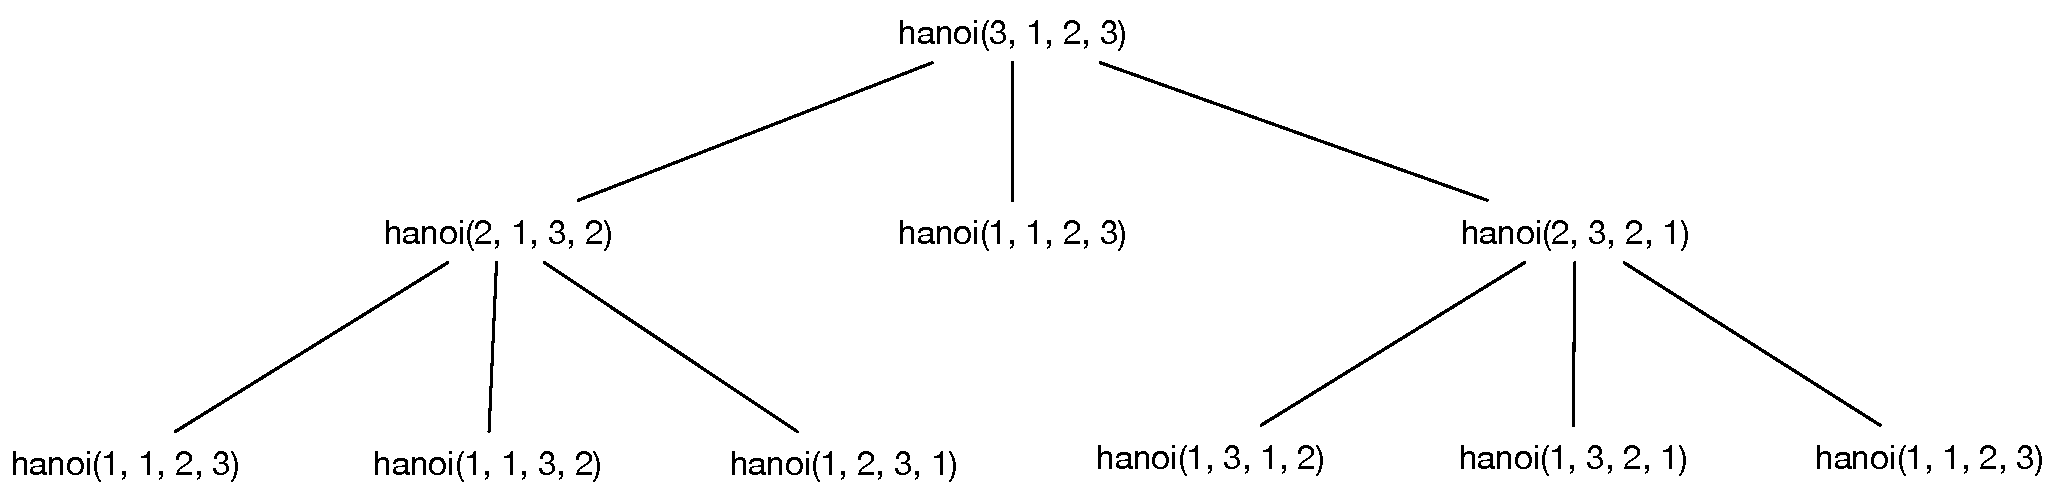
\includegraphics[scale=0.28]{./Figure/elementaryCS-figHanoi-Hint.pdf}
  \end{center}
\end{frame}
\begin{frame}[fragile,shrink]
\frametitle{繰り返しと再帰}
  \begin{itemize}
\item 以前,繰り返しでいろいろな計算を実現しました
\item 再帰は繰り返しに変換できることがあります
\item ここでは繰り返しと再帰の関係について見ていきます
  \end{itemize}
\end{frame}
\subsection{末尾再帰 (Tail Recursion)}
\begin{frame}[fragile,shrink]
\frametitle{末尾再帰呼び出し (Tail Recursive Call)}
  \begin{itemize}
\item どちらも再帰的定義ですが計算プロセスに違いがあります
\item \lstref{fact-rec1} は fact(n) を得るために fact(n-1) の後の計算 (n  $\times\,\Box$) を覚えてなければならない
\item \lstref{fact-iter} はその必要はなく,計算の状態``カウンタと途中までの積''を覚えておくだけで良い
\item \lstref{fact-iter} のような形を末尾再帰的といいます
  \end{itemize}
\vspace{-2em}
  \begin{columns}[t]
    \begin{column}{0.45\textwidth}
      \begin{lstlisting}[caption={再帰プロセス版},label=fact-rec1]
# Factorial
def fact (n):
  if (n == 1):
    return(1)
  else:
    return(n*(fact(n-1)))
      \end{lstlisting}
    \end{column}
    \begin{column}{0.5\textwidth}
      \begin{lstlisting}[firstnumber=16,caption={繰り返しプロセス版},label=fact-iter]
# Factorial
def fact_iter (n):
  def fact_iter1 (prod, cnt, max):
    if cnt > max:
      return(prod)
    else:
      return(fact_iter1(prod*cnt,cnt+1,max))
  return(fact_iter1(1,1,n))
      \end{lstlisting}
    \end{column}
  \end{columns}
\end{frame}
\begin{frame}[fragile]
\frametitle{末尾呼び出し (Tail Call)}
  \begin{itemize}
\scriptsize
\item 末尾再帰は繰り返し {\tt while, for} に書き換えられます
\item 繰り返しは再帰関数の特別な場合と見なせる
\item 再帰は関数を呼び出すたびに資源を消費するが,繰り返しは一定
  \end{itemize}
  \begin{columns}
    \begin{column}{0.5\textwidth}
      \begin{itembox}{再帰プロセス}
\scriptsize
        \begin{verbatim}
  fact(4)
=>(4 * fact(3))
=>(4 * (3 * fact(2)))
=>(4 * (3 * (2 * fact(1))))
=>(4 * (3 * (2 * 1)))
=>(4 * (3 * 2 ))
=>(4 * 6)
=>24
        \end{verbatim}
      \end{itembox}
    \end{column}
    \begin{column}{0.45\textwidth}
      \begin{itembox}{繰り返しプロセス}
\scriptsize
        \begin{verbatim}
  fact-iter(4)
=>fact-iter1( 1,1,4)
=>fact-iter1( 1,2,4)
=>fact-iter1( 2,3,4)
=>fact-iter1( 6,4,4)
=>fact-iter1(24,5,4)
=>24
        \end{verbatim}
      \end{itembox}
    \end{column}
  \end{columns}
\end{frame}
%
%%% COMPUTER
%
\section{コンピュータの中では}
\begin{frame}[shrink]
\frametitle{CPU とメモリ}
  \begin{itemize}
\item コンピュータの命令自体も符号化されてます
\item CPU (Central Processing Unit) ごとに命令セットも符号も異なっています
\item ここでは CPU が命令を実行するサイクルについて見てみます
  \end{itemize}
  \begin{center}
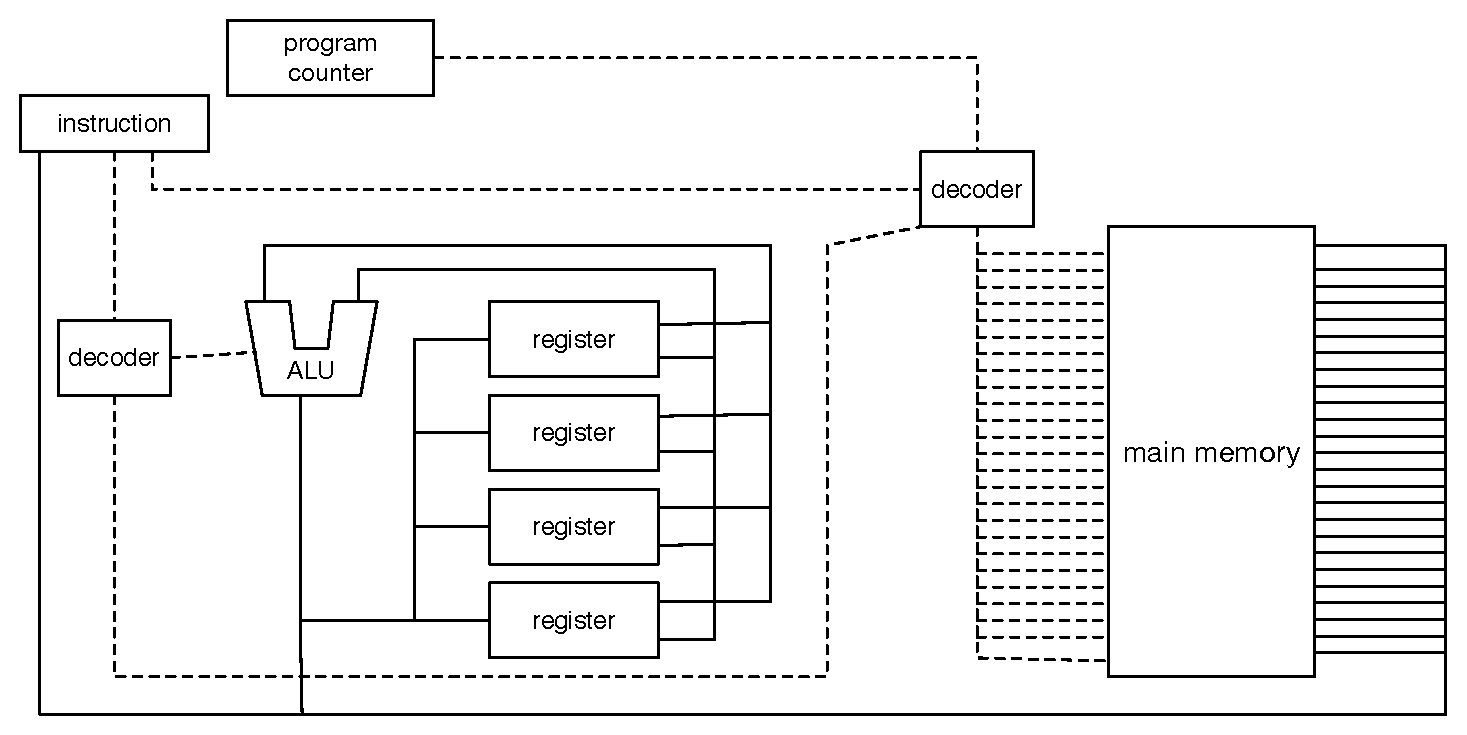
\includegraphics[scale=0.3]{./Figure/elementaryCS-figCPU}
  \end{center}
\end{frame}
\begin{frame}[shrink]
\frametitle{演算のサイクル}
  \begin{enumerate}
\scriptsize
\item Instruction に命令をフェッチ
\item メインメモリからレジスタにデータを移動
\item ALU (Arithmetic and Logic Unit) がレジスタからデータを取り出す
\item ALU で演算
\item 結果をレジスタに書き込む
\item レジスタからメインメモリにデータを移動
\item ADD cx dx bx という命令を例にすると下図のようになります
  \end{enumerate}
  \begin{center}
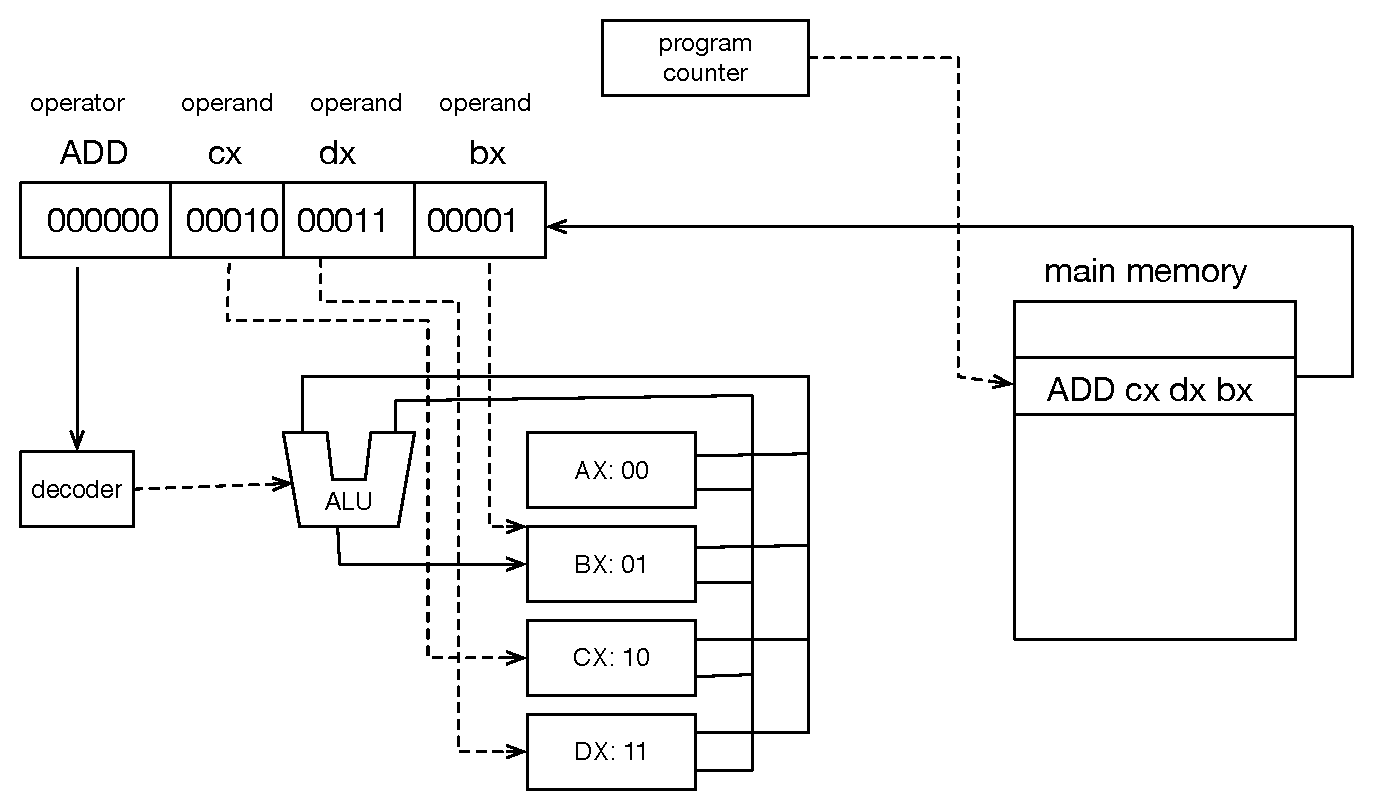
\includegraphics[scale=0.3]{./Figure/elementaryCS-figCycle}
  \end{center}
\end{frame}
\begin{frame}[shrink]
\frametitle{関数を呼び出したとき}
  \begin{itemize}
\item 関数を呼び出すたびに下図の右側のように実行時スタックの領域に保存する
    \begin{itemize}
\item 活性レコード (activation record) という
    \end{itemize}
\item 終了すれば活性レコードは開放される
\item 多くのプログラミング言語は末尾再帰を繰り返しに変換してくれないので繰り返し構文が用意されている
  \end{itemize}
  \begin{center}
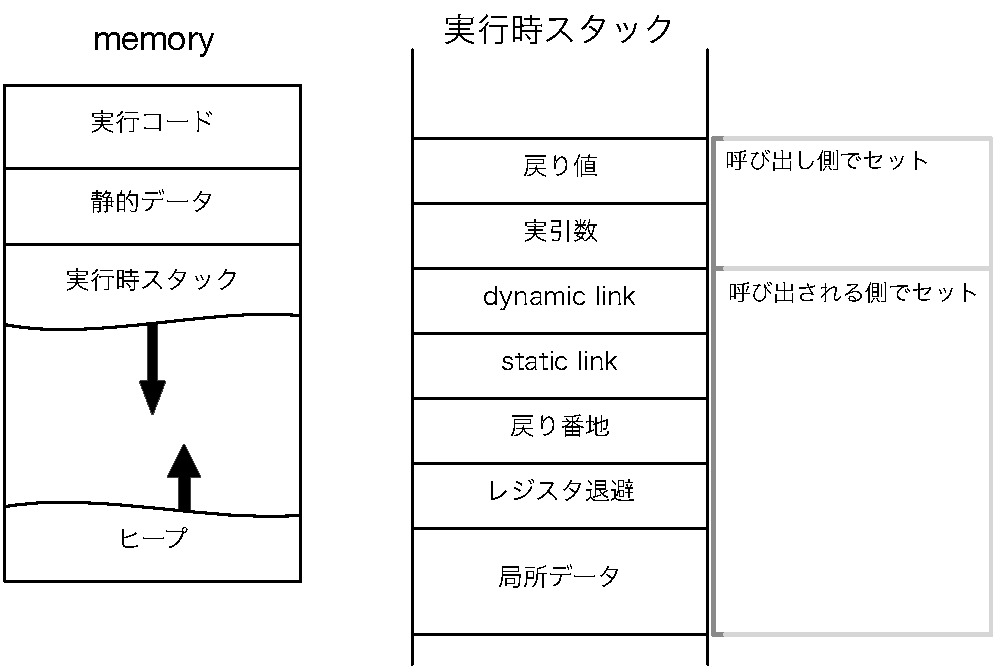
\includegraphics[scale=0.3]{./Figure/elementaryCS-figMemory}
  \end{center}
\end{frame}
\section{再帰のまとめ}
\begin{frame}[fragile]
\frametitle{再帰のまとめ}
  \begin{itemize}
\item 再帰とはある問題をそれより簡単な同じ問題に分解して問題を解く方法
\item 既にわかっているそれより前のものから求める
\item 一見複雑な問題も再帰的に定義すると単純な計算で解ける
\item それ以上分割出来ない問題を解き,結果からより大きい問題の結果を得るというもの (分割統治法 (Divide and Conquer) と呼ばれる)
\item E.g. Quiz 1 では複雑な問題をより小さい同じ問題に分解して解いていっている
\item 再帰は非常に強力な解法になる
  \end{itemize}
\end{frame}

%
%%% SPECIAL QUIZ
%
%\section{課題 S 演習ガイド}
\subsection{課題 S}
\begin{frame}[containsverbatim, shrink, label=quizS]
\frametitle{課題 S}
  \begin{itemize}
\item \href{https://sites.google.com/a/presystems.xyz/sample/home/elementary-computer-science}{\beamerbutton{https://sites.google.com/a/presystems.xyz/sample/home/elementary-computer-science}} から fib-skeleton.py をダウンロード
\item フィボナッチ数を求める問題です
\item まだ,お話していない部分も含まれるのですぐに取り掛からなくていいです
\item ソースコード中のコメントを参照して (2)-(4) の問に答えて見てください
\item 提出は出来たところまででいいです
\item 出来なかったところはコメントにしてください
  \end{itemize}
\end{frame}

%
%%% 実数
%
%\part{大きい数と小さい数の計算}
%\frame{
%  \frametitle{大きい数と小さい数の計算}
%\scriptsize
%  \tableofcontents[part=3]
%}
%\section{数の表現}
\begin{frame}[shrink]
\frametitle{繰り返しや再帰によるその他の計算}
  \begin{itemize}
\item 繰り返しや再帰は自然数 $n$ に対応する解を求めるような感じ
    \begin{itemize}
\item 数列は $n$ 番目の数を求める: \(\alpha\colon N\rightarrow N\)
\item ハノイの塔も $n$ 枚目の解を求める
    \end{itemize}
\item これを利用して関数の解を求める計算に利用する
\item たとえば非線形方程式 \(f(x)=0\) の実根を求める
\item \href{run:newton.command}{\beamerbutton{ニュートン法}}
    \begin{itemize}
\item \(\sqrt{a}\) を求めてみる
\item \(f(x)=x^2-a\) として \(f(x)=0\) となる $x$ を求める
\item \(k+1\) 番目の近似値 \(x_{k+1}\) を
      \begin{displaymath}
x_{k+1} = x_k-\frac{f(x_k)}{f'(x_k)} = \frac{1}{2}(x_k+\frac{a}{x_k})
      \end{displaymath}
で求める
\item \(x_{k+1}\) と \(x_k\) が十分近くなったら停止
    \end{itemize}
  \end{itemize}
\end{frame}
\subsection{非負整数の表現}
\begin{frame}[label=Top_Integer]
\frametitle{非負整数のコンピュータ内での表現}
  \begin{itemize}
\item 10 進数から 2 進数への変換
  \end{itemize}
  \begin{center}
   \begin{example}[10進$\Leftrightarrow$2進]
   \begin{columns}[t]
    \begin{column}{3cm}
\infer[\mbox{High}]{0}{\infer{2)1\cdots 1}{\infer{2)2\cdots 0}{\infer{2)4\cdots 0}{\infer[\mbox{Low}]{2)9\cdots 1}{2)19\cdots 1}}}}}
    \end{column}
    \begin{column}{3cm}
\infer{19}{\infer{1\times 2^4=16}{\infer{0\times 2^3=0}{\infer{0\times 2^2=0}{\infer{1\times 2^1=2}{1\times 2^0=1}}}}}
    \end{column}
   \end{columns}
   \end{example}
  \end{center}
\end{frame}
\subsection{負の数の表現}
\begin{frame}[shrink]
\frametitle{負の数の表現}
  \begin{itemize}
\item 負の数をあらわすには補数表現をもちいます
\item それでは 2 の補数(2's complement) を求めてみましょう
  \end{itemize}
  \begin{block}{2 の補数表現}
    \begin{enumerate}
\item 2 進表記において各ビットを反転する
\item それに 1 を足す
    \end{enumerate}
  \end{block}
  \begin{center}
    \begin{example}[-8$\sim$7 (2 進 4 桁) の 2 の補数表現]
\((1000)_{(2)}\Rightarrow(1001)_{(2)}\Rightarrow(1010)_{(2)}\Rightarrow (1011)_{(2)}\Rightarrow (1100)_{(2)}
\Rightarrow(1101)_{(2)}\Rightarrow(1110)_{(2)}\Rightarrow(1111)_{(2)}
\Rightarrow(0000)_{(2)}\Rightarrow(0001)_{(2)}\Rightarrow(0010)_{(2)}\Rightarrow(0011)_{(2)}
\Rightarrow(0100)_{(2)}\Rightarrow(0101)_{(2)}\Rightarrow(0110)_{(2)}\Rightarrow(0111)_{(2)}\)\\
      \begin{itemize}
\item Successor (1 足す) でつぎの数になるようになっている
\item 最上位ビットがサインビットになっている
\item circulation の実行
      \end{itemize}
    \end{example}
  \end{center}
\end{frame}
\subsection{計算機内の計算}
\begin{frame}[shrink]
\frametitle{計算機内の計算}
\framesubtitle{整数の減算}
  \begin{itemize}
\item 2 進 $n$ 桁の数 $a, b$ (\(A_k,B_k\in\{1,0\}\))
    \begin{itemize}
\item \(a\colon A_{n-1}A_{n-2}\cdots A_{1}A_{0}\)
\item \(b\colon B_{n-1}B_{n-2}\cdots B_{1}B_{0}\)
    \end{itemize}
\item \(a, b\) はそれぞれ
\[a=\sum_{k=0}^{n-1}2^{k}A_{k}\]
\[b=\sum_{k=0}^{n-1}2^{k}B_{k}\]
\item $b$ の各桁を反転させたものを \(\overline{B_{k}}\) として $b$ の補数 \(\overline{b}\) は
\[\overline{b}=\sum_{k=0}^{n-1}2^{k}\overline{B_{k}}=\sum_{k=0}^{n-1}2^{k}(1-B_{k})=(2^n-1)-b\]
  \end{itemize}
\end{frame}
\begin{frame}[shrink]
\frametitle{計算機内の計算\textemdash Cont.}
  \begin{itemize}
\item \(\overline{b}=(2^n-1)-b\) より
    \begin{eqnarray*}
a-b&\Rightarrow& a-((2^n-1)-\overline{b})\\
   &=&a+\overline{b}+1-2^n
    \end{eqnarray*}
\item 引き算は補数を足すことで表す
\item \(\overline{b}+1\) は 2 の補数
\item \(-2^n\) は最上位の桁上がりは無視
  \end{itemize}
  \begin{example}[引き算の例]
    \begin{itemize}
\item 4 桁の2進数と仮定して \(6-3\) と \(3-6\)
    \end{itemize}
    \begin{columns}[t]
      \begin{column}{3.5cm}
        \begin{tabular}{ccccc}
&0&1&1&0\\
$+$&1&1&0&1\\
\hline
&0&0&1&1\\
        \end{tabular}
      \end{column}
      \begin{column}{3.5cm}
        \begin{tabular}{ccccc}
&0&0&1&1\\
$+$&1&0&1&0\\
\hline
&1&1&0&1\\
        \end{tabular}
      \end{column}
    \end{columns}
  \end{example}
\end{frame}

%\subsection{実数の表現}
\begin{frame}[shrink]
\frametitle{実数の表現}
\framesubtitle{浮動小数 (floating point number)}
  \begin{itemize}
\item 浮動小数 \(ab^{e}\)
    \begin{itemize}
\item $a$ は仮数 (significand or coefficient) ,$b$ は底 (base),$e$ は指数 (exponent) と呼ぶ
    \end{itemize}
\item \(\frac{1}{b}\leq|a|<1\) のとき正規浮動小数 (normalized floating point number) と云う
\item 上のような変換を正規化(normalizaiton) と云う
\item 符号,指数,仮数で一意に決定できます
  \end{itemize}
  \begin{example}[正規浮動小数]
   \begin{math}
    \begin{array}{rcl}
1.234 &\Rightarrow& +0.1234\times 10^1\\
-12.34 &\Rightarrow& -0.1234\times 10^2\\
0.01234 &\Rightarrow& +0.1234\times 10^{-2}\\
    \end{array}
   \end{math}
  \end{example}
\end{frame}
\begin{frame}
\frametitle{実数の 2 進表記}
  \begin{itemize}
\item 実数も 2 進表記に変換した上で正規化します
\item 13.6875$_{(10)}$ を2進数へ変換してみます
  \end{itemize}
  \begin{center}
   \begin{example}[10進実数 13.6875$_{(10)}$ を2進数へ]
     \begin{columns}[t]
       \begin{column}{4.5cm}
\infer[High]{0}{\infer{2)1\cdots 1}{\infer{2)3\cdots 1}{\infer[Low]{2)6\cdots 0}{2)13\cdots 1}}}}
         \begin{itemize}
\item 13$_{(10)}$ は 1101$_{(2)}$
         \end{itemize}
       \end{column}
     \begin{column}{4.5cm}
\infer[Low]{.5\times 2=1.00}{\infer{.75\times 2=1.50}{\infer[High]{.375\times 2=0.75}{.6875\times 2=1.375}}}
     \begin{itemize}
\item .6875$_{(10)}$ は .1011$_{(2)}$
     \end{itemize}
      \end{column}
     \end{columns}
     \begin{itemize}
\item ゆえに, 13.6875$_{(10)}$ は 1101.1011$_{(2)}$ となる 
     \end{itemize}
   \end{example}
  \end{center}
\end{frame}
\begin{frame}
\frametitle{実数の 2 進表記 - Cont.}
  \begin{itemize}
\item 得られた 2 進数を正規化します
\item 最上位ビットが 1 になるようにします (注意: 正規化の定義と違っているので注意)
  \end{itemize}
  \begin{center}
    \begin{example}[1101.1011$_{(2)}$ を正規化]
1101.1011$_{(2)}$ \(\Rightarrow\) 0.11011011\(\times 2^4\)
      \begin{itemize}
\item 符号: +
\item 指数: 4
\item 仮数: 0.11011011
      \end{itemize}
    \end{example}
  \end{center}
\end{frame}
\begin{frame}[shrink]
\frametitle{実数の 2 進表記 - Cont.}
  \begin{itemize}
\item 符号,指数,仮数が正規化によって決まります
\item これを 32 ビットで表す
\item 右に小数点を一つ移動
\item 最上位ビットは必ず 1 になるので省略
\item 規格 \href{http://ieeexplore.ieee.org/xpl/mostRecentIssue.jsp?punumber=2355}{\beamerbutton{IEEE 754}} はもうひと段階
  \end{itemize}
  \begin{center}
    \begin{example}[指数部,仮数部]
      \begin{itemize}
\item 1.1011011\(\times 2^3\) の符号,指数,仮数は以下のとおり
        \begin{itemize}
\item 符号 (sign): +
\item 指数 (exponent): 3
\item 仮数 (significand): 1.1011011
        \end{itemize}
      \end{itemize}
    \end{example}
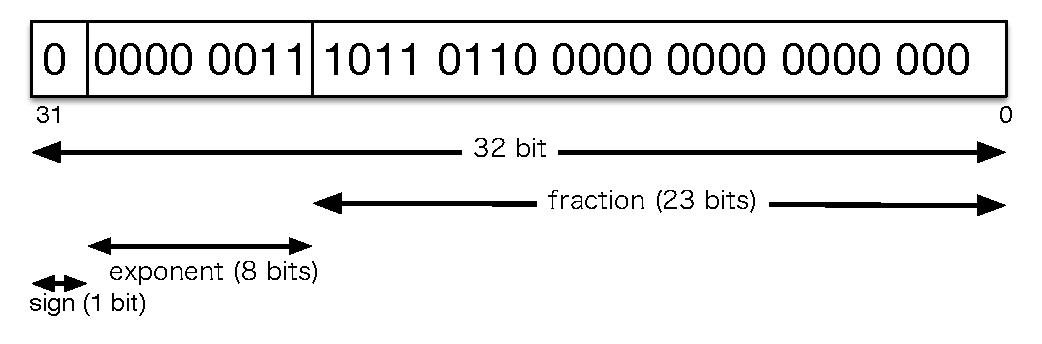
\includegraphics[scale=.4]{./Figure/elementaryCS-figFloatingPointFormat.eps}
  \end{center}
\end{frame}
\begin{frame}
\frametitle{宿題 3: 浮動小数}
  \begin{itemize}
\item 実数の浮動小数表現をやってみてください
  \end{itemize}
  \begin{block}{宿題 3}
    \begin{itemize}
\item 35.75 を浮動小数で表現してみてください
\item T2Schola に小テストがあるのでそれに答えてください
    \end{itemize}
  \end{block}
\end{frame}
\begin{frame}
\frametitle{宿題 3: 回答}
  \begin{itemize}
\item 2 進へ変換: 100011.11
\item 正規化: 1.0001111$\times 2^5$
\item 32 bit 形式に: {\scriptsize 0 0000 0101 0001 1110 0000 0000 0000 000}
    \begin{itemize}
\item 1. は省略
    \end{itemize}
\item 規格\href{http://ieeexplore.ieee.org/xpl/mostRecentIssue.jsp?punumber=2355}{\beamerbutton{IEEE 754}}では下駄 (bais) をはかせるので\(5+127=132\Rightarrow\) 1000 0100
\item 32 bit 形式に: {\scriptsize 0 1000 0100 0001 1110 0000 0000 0000 000}
  \end{itemize}
\end{frame}
\subsection{浮動小数の算術演算}
\begin{frame}[shrink,fragile]
\frametitle{浮動小数演算の変な現象 1}
  \begin{itemize}
\item roundoff.py を実行してみます
\item 結果が予測と少し違うことになります
\item \(0.6_{(10)}\) は \((0.1001\ldots)_{(2)}\), \(0.4_{(10)}\) は \((0.0110\ldots)_{(2)}\), \(0.2_{(10)}\) は \((0.0011\ldots)_{(2)}\) となります
  \end{itemize}
  \begin{lstlisting}[caption={roundoff.py},label=lst:roundoff]
if (float(0.6)-float(0.4)==float(0.2)):
   print("is equal")
else:
   print("not equal")
  \end{lstlisting}
\end{frame}
\begin{frame}[shrink,fragile]
\frametitle{浮動小数演算の変な現象 2}
  \begin{itemize}
\item machine\_epsilon.py を実行してみます
\item 結果が予測と少し違うことになります
\item この原因についてみていきます
  \end{itemize}
  \begin{lstlisting}[caption={machine\_epsilon.py},label=lst:epsilon]
# Machine epsilon
import sys

epsilon, old, prod =1.0, 0.0, 0.0
cnt=0
while (prod!=1.0):
  print(epsilon)
  old = epsilon
  cnt=cnt+1
  epsilon=epsilon/2.0
  prod=epsilon+1.0
print("Calculated machine epsilon:",old)
print("System information in Python:",sys.float_info.epsilon)
  \end{lstlisting}
\end{frame}
\begin{frame}[shrink]
\frametitle{浮動小数数の算術演算}
  \begin{itemize}
\item 正規化した 2 つの浮動小数 \(X, Y\) を \(X=F_x\times 10^{e_x}, Y=F_y\times 10^{e_y}\) とする
\item 乗算: \(XY=(F_x\times 10^{e_x})(F_y\times 10^{e_y})=F_xF_y\times 10^{e_x+e_y}\)
\item 除算: \(\frac{X}{Y}=\frac{(F_x\times 10^{e_x})}{(F_y\times 10^{e_y})}=\frac{F_x}{F_y}\times 10^{e_x-e_y}\)
\item 加算\(\cdot\)減算: \(X\pm Y=(F_x\times 10^{e_x})\pm(F_y\times 10^{e_y})=(F_x\pm F_y\cdot 10^{e_y-e_x})\times 10^{e_x}\)
    \begin{itemize}
\item ただし,\(e_x\geq e_y\)
\item \(F_y\cdot 10^{e_y-e_x}\) は指数を大きい方に揃えたときの $Y$ の仮数
    \end{itemize}
\item 演算結果も正規化するので指数は調整が必要
  \end{itemize}
  \begin{example}[算術演算の例]
    \begin{columns}[t]
      \begin{column}{4.5cm}
        \begin{math}
          \begin{array}{cll}
&0.2184&\times 10^2\\
\times&0.2512&\times 10^2\\
\hline
&0.07998208&\times 10^4\\
=&0.7998208&\times 10^3\\
          \end{array}
        \end{math}
      \end{column}
      \begin{column}{4.5cm}
        \begin{math}
          \begin{array}{cll}
&0.2844&\times 10^3\\
+&0.4162&\times 10^1\\
\hline
&0.288562&\times 10^3\\
          \end{array}
        \end{math}
      \end{column}
    \end{columns}
  \end{example}
\end{frame}
%\begin{frame}
%\frametitle{算術演算の誤差}
%  \begin{itemize}
%\item 4 桁までしか記憶できないと仮定
%\item \(0.2844\cdot 10^3+0.4162\cdot 10^1=0.288562\cdot 10^3=(0.2885+0.000062)\cdot 10^3=0.2885\cdot 10^3+0.6200\cdot 10^{-1}\)
%\item \(0.288562\)が真の値となるが \(0.2885\) までしか記憶できないので
%\item \(0.6200\cdot 10^{-1}(=0.000062\cdot 10^3)\) について調整する必要がある
%  \end{itemize}
%  \begin{example}[\(0.2844\cdot 10^3+0.4162\cdot 10^1\)]
%    \begin{columns}[t]
%      \begin{column}{4.5cm}
%        \begin{math}
%          \begin{array}{cll}
%&0.2844&\times 10^3\\
%+&0.4162&\times 10^1\\
%\hline
%&0.288562&\times 10^3\\
%          \end{array}
%        \end{math}
%      \end{column}
%      \begin{column}{4.5cm}
%        \begin{math}
%          \begin{array}{cll}
%&0.2844&\times 10^3\\
%+&0.004162&\times 10^3\\
%\hline
%&0.288562&\times 10^3\\
%          \end{array}
%        \end{math}
%      \end{column}
%    \end{columns}
%  \end{example}
%\end{frame}
\section{誤差のおはなし}
\subsection{丸め誤差 (roundoff error)}
\begin{frame}[shrink]
\frametitle{誤差とは}
  \begin{itemize}
\item コンピュータの中では実数は有限個の 0 と 1 の組み合わせ(浮動小数)で表しています
\item なので,本来あるべき真値を適当な浮動小数で近似している
\item 近似値-真値 を誤差という
  \end{itemize}
\end{frame}
\begin{frame}[shrink]
\frametitle{丸め誤差 (roundoff error)}
  \begin{itemize}
\item 表現可能な範囲に丸めることを丸め誤差という(\lstref{lst:roundoff}参照)
\item 演算結果も丸める
\item $Z$ を演算結果とする
\item $d$ 桁だけ記憶できるとして,先頭の $d$ 桁を $F$,残りを $f$ とすると,\(Z=F\cdot 10^{e_z}+f\cdot 10^{e_z-d}\)
\item $f$ の値で四捨五入することにして
    \begin{displaymath}
      \begin{array}{ll}
|f|<0.5 \mbox{のとき} & |Z|=|F|\cdot 10^{e_z-d}\\
|f|\geq 0.5 \mbox{のとき} & |Z|=|F|\cdot 10^{e_z-d}+\cdot 10^{e_z-d}
      \end{array}
    \end{displaymath}
\item 丸め誤差 $\epsilon_z$ とすれば
    \begin{displaymath}
      \begin{array}{ll}
|f|<0.5 \mbox{のとき} & |\epsilon_z|=|f|\cdot 10^{e_z-d}\\
|f|\geq 0.5 \mbox{のとき} & |\epsilon_z|=|1-f|\cdot 10^{e_z-d}
      \end{array}
    \end{displaymath}
  \end{itemize}
  \begin{example}[\(0.2844\cdot 10^3+0.4162\cdot 10^1\)]
    \begin{itemize}
\item \(0.2844\cdot 10^3+0.4162\cdot 10^1=0.2885\cdot 10^3+0.6200\cdot 10^{-1}\)
\item \(|Z|=0.2885\cdot 10^3+10^{3-4}=0.2886\cdot 10^3\)
\item \(|\epsilon_z|=|1-0.6200|\cdot 10^{3-4}=0.48\cdot 10^{-1}\)
    \end{itemize}
  \end{example}
\end{frame}
%\begin{frame}
%\frametitle{相対誤差 (relative error)}
%  \begin{itemize}
%\item 計算のコストだけでなくときには計算精度も重要になる
%\item 真の値 $x^t$,観測した値 $x$ として誤差 \(\epsilon_x=x^t-x\)
%\item \(|\epsilon_x|=|x^t-x|\) を絶対誤差という
%\item 相対誤差 \(r_x=\frac{\epsilon_{x}}{x}=\frac{x^t-x}{x}\) で精度を測る
%  \end{itemize}
%  \begin{example}[相対誤差の例]
%    \begin{itemize}
%\item \(x_t=9, x=10\) と \(y_t=999, y=1000\) の場合を考える
%\item $x$ と $y$ の誤差はどちらも \(-1\)
%\item $x$ と $y$ の相対誤差はそれぞれ \(r_x=\frac{-1}{10}, r_y=\frac{-1}{1000}\)
%    \end{itemize}
%  \end{example}
%\end{frame}
%\subsection{誤差の伝搬 (propagation of errors)}
%\begin{frame}
%\frametitle{誤差の伝搬 (propagation of errors)}
%  \begin{itemize}
%\item 誤差は計算中伝播して計算結果を不正確にしてしまう
%\item 算術式中の誤差がどう蓄積されていくかをみる
%\item ある数 $x, y$ としてそれぞれが誤差 \(\epsilon_x, \epsilon_y\) を持つとする
%\item このときの演算 \(x\oplus y\) の誤差 \(\epsilon_{x\oplus y}\) は
%    \begin{displaymath}
%\epsilon_{x\oplus y}=(x^t\oplus y^t)-(x\oplus y)
%    \end{displaymath}
%\item \(x^t\oplus y^t\) は真の演算結果で, \(x\oplus y\) は実際の結果
%\item 先の誤差の定義からこれが導ける
%  \end{itemize}
%\end{frame}
%\begin{frame}[shrink]
%\frametitle{誤差公式}
%  \begin{itemize}
%\item 各演算についてつぎの関係が成り立つ
%  \end{itemize}
%  \begin{theorem}[誤差公式]
%    \begin{math}
%      \begin{array}{lclclclcl}
%\scriptsize
%\epsilon_{x+y}&=&(x^t+y^t)-(x+y)&=&(x^t-x)+(y^t-y)&=&\epsilon_x+\epsilon_y\\
%\epsilon_{x-y}&=&(x^t-y^t)-(x-y)&=&(x^t-x)-(y^t-y)&=&\epsilon_x-\epsilon_y\\
%      \end{array}
%    \end{math}
%    \begin{math}
%      \begin{array}{lclclclcl}
%\epsilon_{xy}&=&(x^ty^t)-(xy)&=&(x+\epsilon_x)(y+\epsilon_y)-(xy)&=&\epsilon_x y+\epsilon_y x\\
%      \end{array}
%    \end{math}
%    \begin{math}
%      \begin{array}{lclclclcl}
%\epsilon_{\frac{x}{y}}&=&\frac{x^t}{y^t}-\frac{x}{y}&=&\frac{x^ty-y^tx}{y^ty}&=&\frac{(x+\epsilon_x)y-(y+\epsilon_y)x}{(y+\epsilon_y)y}\\
%&=&\frac{xy+\epsilon_xy-xy+x\epsilon_y}{y^2(1+\frac{\epsilon_y}{y})}&=&\frac{\epsilon_xy-\epsilon_yx}{y^2}\\
%      \end{array}
%    \end{math}
%    \begin{itemize}
%\item \(\epsilon_x\epsilon_y\) は十分小さいとして無視
%\item \(|\frac{\epsilon_y}{y}|\) は \(|\frac{\epsilon_y}{y}|\ll 1\) のとき無視
%\item これに各演算の丸め誤差 \(\alpha\) を加えたて誤差公式とする
%      \begin{itemize}
%\item たとえば 4 桁までしか記憶できないのであれば演算結果も 4 桁に丸められる
%      \end{itemize}
%    \end{itemize}
%  \end{theorem}
%\end{frame}
%\begin{frame}[shrink]
%\frametitle{相対誤差公式}
%  \begin{itemize}
%\item 相対誤差公式を導く
%\item 先の相対誤差の定義より
%    \begin{displaymath}
%r_{x\oplus y}=\frac{\epsilon_{x\oplus y}}{x\oplus y}
%    \end{displaymath}
%\item とすれば誤差公式よりつぎの相対誤差公式をえる
%  \end{itemize}
%  \begin{theorem}[相対誤差公式]
%    \begin{math}
%      \begin{array}{rclcl}
%r_{x+y}&=&\frac{\epsilon_x+\epsilon_y}{x+y}+\alpha&=&r_x\frac{x}{x+y}+r_y\frac{y}{x+y}+\alpha\\
%r_{x-y}&=&\frac{\epsilon_x-\epsilon_y}{x-y}+\alpha&=&r_x\frac{x}{x-y}+r_y\frac{-y}{x-y}+\alpha\\
%r_{xy}&=&\frac{\epsilon_x y+\epsilon_y x}{xy}+\alpha&=&r_x\ 1+r_y\ 1+\alpha\\
%r_{xy}&=&\frac{\frac{\epsilon_x y-\epsilon_y x}{y^2}}{\frac{x}{y}}+\alpha&=&r_x\ 1+r_y\ (-1)+\alpha
%      \end{array}
%    \end{math}
%  \end{theorem}
%\end{frame}
%\begin{frame}[shrink]
%\frametitle{誤差伝播の解析}
%  \begin{itemize}
%\item 相対誤差公式を使って誤差伝播の解析を行う
%  \end{itemize}
%  \begin{example}[和における誤差伝播]
%    \begin{itemize}
%\item \(r_0, r_1, r_2, r_3\) を実数 \(a_0,a_1,a_2,a_3\) の相対誤差とする
%\item \(S=(((a_0+a_1)+a_2)+a_3)\) の相対誤差を求める
%    \end{itemize}
%  \end{example}
%\end{frame}
\subsection{情報落ち誤差}
\begin{frame}[shrink]
\frametitle{情報落ち誤差(loss of trailing digits)}
  \begin{itemize}
\item 絶対値が大きく異なる 2 つの数の加減算では小さい数が無視されることがある
\item \lstref{lst:epsilon} で見たような場合
  \end{itemize}
\end{frame}
\subsection{打ち切り誤差 (truncation error)}
\begin{frame}[shrink]\label{sl:back}
\frametitle{打ち切り誤差 (truncation error)}
  \begin{itemize}
\item コンピュータでは無限に繰り返して値をもとめることはできない
\item 有限回の計算で値を計算し,それを求める値の近似値としてもちいる
\item このときの誤差を打切り誤差という
  \end{itemize}
  \begin{example}[\(\sin(x)\)のマクローリン展開]
    \begin{itemize}
\item \(sin(x)=x-\frac{x^3}{3!}+\frac{x^5}{5!}-\frac{x^7}{7!}+\cdots+(-1)^{n}\frac{x^{2n+1}}{(2n+1)!}+\cdots\)
\item gnuplot で試してみてください
    \end{itemize}
  \end{example}
  \begin{example}[平方根の計算]
    \begin{itemize}
%\item \href{run:newton.command}{\beamerbutton{ニュートン法}}
\item newton.py を参照\hyperlink{newton-is_enough-rec}{\beamerbutton{プログラム例}}
\item \(\sqrt{a}\) を求めてみる
\item \(f(x)=x^2-a\) として \(f(x)=0\) となる $x$ を求める
\item \(k+1\) 番目の近似値 \(x_{k+1}\) を
      \begin{displaymath}
x_{k+1} = x_k-\frac{f(x_k)}{f'(x_k)} = \frac{1}{2}(x_k+\frac{a}{x_k})
      \end{displaymath}
    \end{itemize}
  \end{example}
\end{frame}
%\section{まとめ}
%\begin{frame}[shrink,fragile]
%\frametitle{数値計算}
%  \begin{itemize}
%\item ここで取り上げたおはなしは数値計算(計算機科学の一分野)のなかの計算誤差をとりあげたもの
%\item シミュレーションなどではある関数の実際の数値を必要とする場合がある
%    \begin{itemize}
%\item 例えば,方程式 \(f(x)=0\) の $x$ を数値的に求める
%    \end{itemize}
%\item 数値計算の手順
%    \begin{itemize}
%\item 最初に適当な 1 次近似 \(x_0\) を選んで,
%\item より良い近似を求め,
%\item 適当な収束条件を満たすまで繰り返す (マシンイプシロンは収束条件の重要な指標)
%    \end{itemize}
%\item \(f\) は複雑なので数値的な解を求めるいろいろな算法を考察
%  \end{itemize}
%\end{frame}

%
%%% アルゴリズム
%
\part{アルゴリズム}
\frame{
  \frametitle{よいアルゴリズム,わるいアルゴリズム,ふつうのアルゴリズム}
\scriptsize
  \tableofcontents[part=3]
}
\section{良いアルゴリズム,わるいアルゴリズム}
\subsection{アルゴリズムとは}
\begin{frame}[containsverbatim, shrink]
\frametitle{アルゴリズム}
  \begin{itemize}
\item 前回まで再帰関数についてお話しました
\item これはアルゴリズム的に計算可能という概念を定義する上で重要な役割をします
\item 関数 \(f:D^n\rightarrow D\) が計算可能とは,それを計算するアルゴリズム(算法)が存在すること
    \begin{itemize}
\item アルゴリズムとは停止する命令の有限の列をいう
\item コンピュータにプログラムできるなにがしか
    \end{itemize}
\item たとえば,
    \begin{itemize}
\item $D$ は最小(あるは極小)があって並んでいるという構造を持つ
\item \(x\in D\) として \(f(x)=G(f\upharpoonright x)\)
\item $D$ を自然数すれば \((N;0,S,+,-,\times,\div,\mathrm{mod},<)\)
\item $G$ を \(0,S,+,-,\times,\div,\mathrm{mod},<\) の有限の列として構成
    \end{itemize}
\item 別の方法として Turing machine を紹介(ホワイトボードに書きます)
\item 計算可能な関数のクラスも理論的に興味深いが,それは別の機会
  \end{itemize}
\end{frame}
\begin{frame}
\frametitle{良いアルゴリズム}
  \begin{itemize}
\item ここでは,すでに計算可能な関数のクラスがあって,その計算の複雑さについて議論する
\item 計算のやり方には良い方法とわるい方法がある
\item 良い方法というのは少ない計算で目的の値を求めること
\item 良い悪いの尺度のひとつ時間計算量について見ていく
\item \(0,S,+,-,\times,\div,\mathrm{mod},<\) のような演算が何回必要かを測る
\item 単にプログラムが動けばいいでなくて
  \end{itemize}
\end{frame}
\subsection{最大公約数を例に導入}
\begin{frame}
\frametitle{まずは最大公約数}
  \begin{itemize}
\item 関数 GCD をふたつの自然数の公約数のうち最大のもの
\item アルゴリズムでは具体的に最大公約数をもとめる計算の仕方を議論する
\item 計算の仕方はいくつか考えられる
    \begin{itemize}
\item アルゴリズムの書き方の自然言語で書いたりいろいろ
    \end{itemize}
  \end{itemize}
  \begin{columns}[t]
    \begin{column}{0.5\textwidth}
      \begin{block}{素朴な方法}
ふたつの整数 \(x, y\) について $1$ から順に \(\min(x,y)\) まで
割って,割り切れる最大の整数
      \end{block}
    \end{column}
    \begin{column}{0.5\textwidth}
      \begin{block}{ユーグリッドの互除法}
\scriptsize
\(x, y\) の最大公約数は $x$ を $y$ で割ったときの剰余と $y$ の最大公約数に等しい
%\setlength{\abovedisplayskip}{10pt}
        \begin{displaymath}
          \begin{array}{rcl}
x_1 &=& n_1 x_2 + x_3\\
x_2 &=& n_2 x_3 + x_4\\
x_3 &=& n_3 x_4 + x_5\\
&\vdots&
          \end{array}
        \end{displaymath}
      \end{block}
    \end{column}
  \end{columns}
\end{frame}
\begin{frame}[fragile,shrink]
\frametitle{最大公約数 (Greatest Common Divisor) のプログラム}
  \begin{itemize}
\item それぞれの実行時間を比較するので見ていてください
    \begin{itemize}
\item 適当な数字思いつかないので
\item 10,000,000 と 10,203,040 の最大公約数
\item 62979284285501 と 62873258567731 の最大公約数
    \end{itemize}
  \end{itemize}
  \begin{columns}[t]
    \begin{column}{0.45\textwidth}
      \begin{lstlisting}[caption={Naive Algorithm}]
def gcd(x,y):
  def min(x,y):
    if (x>y):
      return y
    else:
      return x
  gcm=1
  n=min(x,y)
  for i in range(1,n+1):
    if (x%i==0) and (y%i==0):
      gcm=i
  return (gcm)
      \end{lstlisting}
    \end{column}
    \begin{column}{0.45\textwidth}
      \begin{lstlisting}[caption={Euclidean Algorithm},label=lst:euclid]
def euclid1(x1,x2):
  if x2==0:
    return (x1)
  else:
    return (euclid1(x2,x1%x2))
def euclid(x1,x2):
  def swap(x1,x2):
    return x2,x1
  if (x1<x2) : x1,x2 = swap(x1,x2)
  return(euclid1(x1,x2))
      \end{lstlisting}
    \end{column}
  \end{columns}
\end{frame}
\begin{frame}[fragile]
\frametitle{実行時間の違いについての考察}
  \begin{itemize}
\item Naive な方法
    \begin{itemize}
\item mod や比較の回数を数えてみる
\item $n$ 回で $n$ は $x$ か $y$ の小さい方になっている
    \end{itemize}
\item ユーグリッドの互除法
    \begin{itemize}
\item $n$ よりは少ない回数で計算できる
    \end{itemize}
  \end{itemize}
  \begin{columns}[t]
    \begin{column}{0.45\textwidth}
      \begin{itembox}{euclid(32204,14744)}
\scriptsize
        \begin{verbatim}
  euculid(32204,14744)
=>euclid1(14744,2656)
=>euclid1(2656,1162)
=>euclid1(1162,332)
=>euclid1(332,166)
=>euclid1(166,0)
=>166
        \end{verbatim}
      \end{itembox}
    \end{column}
    \begin{column}{0.45\textwidth}
      \begin{itembox}{euclid(34,21)}
\scriptsize
        \begin{verbatim}
  euculid(34,21)
=>euclid1(21,13)
=>euclid1(13,8)
=>euclid1(8,5)
=>euclid1(5,3)
=>euclid1(3,2)
=>euclid1(2,1)
=>euclid1(1,0)
=>1
        \end{verbatim}
      \end{itembox}
    \end{column}
  \end{columns}
\end{frame}
\begin{frame}[fragile]
\frametitle{ユーグリッドの互除法の演算回数の見積もり}
  \begin{itemize}
\item 最悪の場合について考える
\item 割り算の商がいつまでも 1 であるとき最悪になる
\item となり合う 2 つの Fibonacci 数のとき最悪になる
\item 下の図で $q_i=1$ としたとき Fibonacci 数そのもの
  \end{itemize}
  \begin{columns}[t]
    \begin{column}{0.45\textwidth}
\centering
      \begin{math}
        \begin{array}{rcl}
a_1 &=& q_1 a_2 + a_3\\
a_2 &=& q_2 a_3 + a_4\\
a_3 &=& q_3 a_4 + a_5\\
&\cdots&\\
a_{k-2} &=& q_k a_{k-1}
        \end{array}
      \end{math}
    \end{column}
    \begin{column}{0.45\textwidth}
    \end{column}
  \end{columns}
\end{frame}
\newcommand{\fib}{\mathop{\mathrm{fib}}\nolimits}
\begin{frame}[fragile]
\frametitle{ユーグリッドの互除法の演算回数}
  \begin{itemize}
\item 計算に $k$ 回必要ならば,小さい数は $k$ 番目の Fibonacci 数であるかそれより大きい
\item この定理から小さい方の数を $N$ として
  \end{itemize}
  \begin{center}  
    \begin{math}
      \begin{array}{rcl}
N&\geq& \fib(k)\\
N&\geq& \frac{\phi^{k}}{\sqrt{5}}\ (\mbox{where }\phi=\frac{(1+\sqrt{5})}{2})\\
\log_{\phi}(N)&\geq& \log_{\phi}(\frac{\phi^{k}}{\sqrt{5}})\\
\log_{\phi}(N)+\log_{\phi}\sqrt{5}&\geq& \log_{\phi}\phi^{k}\\
\log_{5}(N)+\log_{5}\sqrt{5}&\geq& k\\
\log_{5}(N)+\frac{1}{2}&\geq& k
      \end{array}
    \end{math}
% 2018 年度は Lame の定理のに変更
  \end{center}
  \begin{itemize}
\item Naive な方法の演算回数 N 回 よりは少ない
  \end{itemize}
\end{frame}
\subsection{べき乗のアルゴリズム}
\begin{frame}[fragile,shrink]
\frametitle{Quiz2: べき乗 (Power) の計算}
  \begin{itemize}
\item 下の例を参考にべき乗を求める良いアルゴリズムを考えてみてください
\item \(b^8\) を求めるのに乗算を 8 回と 3 回
\item ふつうの子より 3 回の方が良い子
\item power-skeleton.py が\href{https://sites.google.com/a/presystems.xyz/sample/home/elementary-computer-science}{\beamerbutton{https://sites.google.com/a/presystems.xyz/sample/home/elementary-computer-science}} に置いてあるので,
ループに変更して実行時間を比較してみてください
\item 提出はいつもの OCW-i からソースコードを提出
  \end{itemize}
  \begin{example}[\(b^8\) の計算]
  \begin{columns}[t]
    \begin{column}{0.55\textwidth}
\(b\times(b\times(b\times(b\times(b\times(b\times(b\times b))))))\)
    \end{column}
    \begin{column}{0.35\textwidth}
\centering
      \begin{math}
        \begin{array}{rcl}
b^2 &=& b \times b\\
b^4 &=& b^2 \times b^2\\
b^8 &=& b^4 \times b^4
        \end{array}
      \end{math}
    \end{column}
  \end{columns}
  \end{example}
\end{frame}
\begin{frame}[fragile,shrink]
\frametitle{べき乗 (Power) のヒント}
  \begin{itemize}
\item 指数は偶数のとき半分に,奇数のとき $-1$ 減る
  \end{itemize}
  \begin{columns}
    \begin{column}{0.45\textwidth}
      \begin{math}
        \begin{array}{rcl}
b^n &=& (b^{\frac{n}{2}})^{2}\\
&& n \mbox{が偶数のとき}\\
b^n &=& b \times b^{n-1}\\
&& n \mbox{が奇数のとき}
        \end{array}
      \end{math}
    \end{column}
    \begin{column}{0.5\textwidth}
      \begin{lstlisting}[caption={power.py},label=fast_power]
def fast_power(b,n):
  def square(x):
    return(x*x)
  def is_even(n):
    if (n%2==0):
      return(True)
    else:
      return(False)
  if (n==1):
    return(b) 
  else:
    if (is_even(n)):
      return(square(fast_power(b,n/2)))
    else:
      return((b*fast_power(b,n-1)))
      \end{lstlisting}
    \end{column}
  \end{columns}
\end{frame}
\section{時間計算量}
\subsection{Big\textendash O Notation}
\begin{frame}[shrink]
\frametitle{時間計算量}
  \begin{itemize}
\item アルゴリズムの良し悪しを測る尺度についてみていきます
\item 良し悪しの基準
    \begin{itemize}
\item 良いアルゴリズム,わるいアルゴリズムを実行時間を計測して比較
\item 入力に対し結果を得るまでの演算 (四則演算や比較演算) の実行回数を見積もって比較
    \end{itemize}
\item 実行時間は CPU や演算の実現方式に依存し計算しようとすると複雑な式になってしまう
\item 演算回数 (時間計算量という)をもとに単純な式で見積もることにする
    \begin{itemize}
\item CPU や実現方式といったものは無視
    \end{itemize}
\item 実行時間がどう変化するかの傾向を見積もれれば十分
  \end{itemize}
  \begin{example}
入力サイズ $n$ として一方は \(100n^2\) ,もう一方は \(n^3\) 回演算を行うとすれば,
 $n$ が十分に大きいときには前者の方が良い
  \end{example}
\end{frame}
\begin{frame}[shrink]
\frametitle{Big\textendash$O$ 記法}
  \begin{itemize}
\item $n$ を入力のサイズとして,演算回数 \(f(n)\) で傾向をつかむ
  \end{itemize}
  \begin{definition}
2 つの関数 \(f, g\colon N\rightarrow R^{>0}\) とする.
    \begin{center}
\(\forall n>k\colon f(n)\leq c\cdot g(n)\)
    \end{center}
となるような \(c, k\) が存在するならば \(f(n)=O(g(n))\) とする
  \end{definition}
  \begin{example}
\(f(n)=n^2+2n+1\) は,たとえば \(c=4, k=1\) として \(f(n)=4\cdot n^2\),よって \(f(n)\) は \(O(n^2)\) となる.
  \end{example}
\end{frame}
\begin{frame}[shrink]
\frametitle{\(f(n)=n^2+2n+1\) は \(O(n^2)\)}
  \begin{itemize}
\item \(n>1\)(=\(k\)) で \(2n\leq 2n^2, 1\leq n^2\) なので
    \begin{displaymath}
0\leq n^2+2n+1\leq n^2+2n^2+n^2= 4n^2
    \end{displaymath}
\item \(c=4, k=1, g(n)=n^2\) となる.よって,
\item \(f(n)=n^2+2n+1<4\cdot n^2\)\ \textemdash\{\(f(n)\leq c\cdot g(n)\)\}
\item \(n\leq 2\) とすると \(2n<n^2, 1<n^2\) 
    \begin{displaymath}
0\leq n^2+2n+1\leq n^2+n^2+n^2= 3n^2
    \end{displaymath}
  \end{itemize}
  \begin{center}
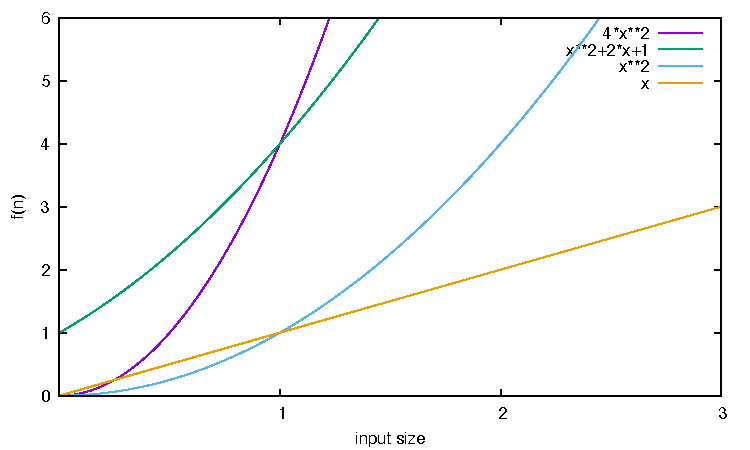
\includegraphics[scale=0.6]{./progs/witness.pdf}
  \end{center}
\end{frame}
\begin{frame}[shrink]
\frametitle{ユーグリットの互除法とべき乗のアルゴリズムのオーダ}
  \begin{example}[ユーグリットの互除法]
    \begin{itemize}
\item Lame の定理: 計算に $k$ ステップ必要ならば,小さい数は $k$ 番目の Fibonacci 数であるかそれより大きい
    \end{itemize}
    \begin{center}  
      \begin{math}
        \begin{array}{rcl}
\fib(n)&=&\frac{\phi^{n}}{\sqrt{5}}\\
&=&\log_{5}(n)+\frac{1}{2}\\
&=&\frac{1}{\log 5}\cdot\log n+\frac{1}{2}<c\log n=O(\log n)
        \end{array}
      \end{math}
    \end{center}
  \end{example}
  \begin{example}[べき乗]
    \begin{itemize}
\item 指数を $n$,2 進表記の 1 の数 $k$,偶数のときはいつも半分になるので $m$ 回偶数が出現するとして,
    \end{itemize}
    \begin{center}
      \begin{math}
        \begin{array}{rcl}
n&=&2^m\\
\log_2 n &=& m
        \end{array}
      \end{math}
    \end{center}
よって, \(f(n)=(\log_2 n)+(k-1)=\frac{1}{\log 2}\cdot\log n+(k-1)<c\log n=O(\log n)\).
  \end{example}
\end{frame}
\begin{frame}[containsverbatim,shrink]
\frametitle{べき乗 (Power) の演算回数の見積もり}
  \begin{itemize}
\scriptsize
\item 各繰り返しで掛け算の回数は 1 回
\item 偶数は何回出てくるか,奇数は何回出てくるかを数える
\item $n$ を指数, $m$ を\(\frac{1}{2}\) する回数として \(\frac{n}{2^m}=1\)
\item そのうち,何回奇数が出てくるかは $n$ を二進表記した時の 1 の数による
    \begin{itemize}
\scriptsize
\item \(\frac{1}{2}\) するとは右に 1 ビットシフト
\item 最下位ビットが 1 のとき奇数
\item 最後 1 乗は計算しないので(1 の数)-1
    \end{itemize}
\item \(\lfloor\log_2 1000\rfloor+5\)=14 回
  \end{itemize}
  \begin{columns}
    \begin{column}{0.45\textwidth}
      \begin{block}{偶数の出現回数}
        \begin{itemize}
\item 二進表記にした時の桁数
        \end{itemize}
        \begin{math}
          \begin{array}{c}
\frac{n}{2^m}=1\\
n=2^m\\
\log_2 n = m
          \end{array}
        \end{math}
      \end{block}
    \end{column}
    \begin{column}{0.5\textwidth}
      \begin{block}{奇数の出現回数}
\scriptsize
        \begin{math}
          \begin{array}{cl}
(1000)_{10}=&(1111101000)_{2}\\
&\Rightarrow_{\frac{1}{2}}0111110100\\
&\Rightarrow_{\frac{1}{2}}0011111010\\
&\Rightarrow_{\frac{1}{2}}0000111110\\
&\Rightarrow_{\frac{1}{2}}0000011111\\
&\cdots\\
&\Rightarrow_{\frac{1}{2}}0000000011
          \end{array}
        \end{math}
      \end{block}
    \end{column}
  \end{columns}
\end{frame}
%\begin{frame}[shrink]
%\frametitle{Big\textendash$\Omega$}
%  \begin{itemize}
%\item Big\textendash$O$ は,``それより大きくなることはない''ということ
%\item では``それより小さくなることはない''ということは ?
%  \end{itemize}
%  \begin{definition}
%2 つの関数 \(f, g\colon N\rightarrow R^{>0}\) とする.
%    \begin{center}
%\(\forall n>k\colon f(n)\geq c\cdot g(n)\)
%    \end{center}
%となるような \(c, k\) が存在するならば \(f(n)=\Omega(g(n))\) とする
%  \end{definition}
%  \begin{block}{オーダ (order)}
%    \begin{itemize}
%\item \(f(n)=O(g(n))\) かつ \(f(n)=\Omega(g(n))\) のとき \(f(n)\) は オーダ \(g(n)\) という
%\item あるいは \(f(n)=O(g(n))\) かつ \(g(n)=O(f(n))\) のとき
%\item e.g. \(n^2+2n+1=O(n^2)\) で \(n^2=O(n^2+2n+1)\) である
%    \end{itemize}
%  \end{block}
%\end{frame}
\section{Sorting}
\begin{frame}[shrink]
\frametitle{Sorting}
  \begin{itemize}
\item Sorting は 2 つの要素の比較と入れ替えだけを用いて,
与えられた集合の要素のリストを昇順(降順)に並べたリストを作ること
\item 例えば \{3,2,4,1,5\} と与えられていれば \{1,2,3,4,5\} と並べたリストを作成する
\item データベースシステムなど多くの場面で利用されている
\item 多くのアルゴリズムが提案されている
\item ここではバブルソート (bubble sort),挿入ソート (insertion sort),クイックソート (quick sort) を紹介する
  \end{itemize}
\end{frame}
\begin{frame}[shrink]
\frametitle{Bubble Sort}
  \begin{center}
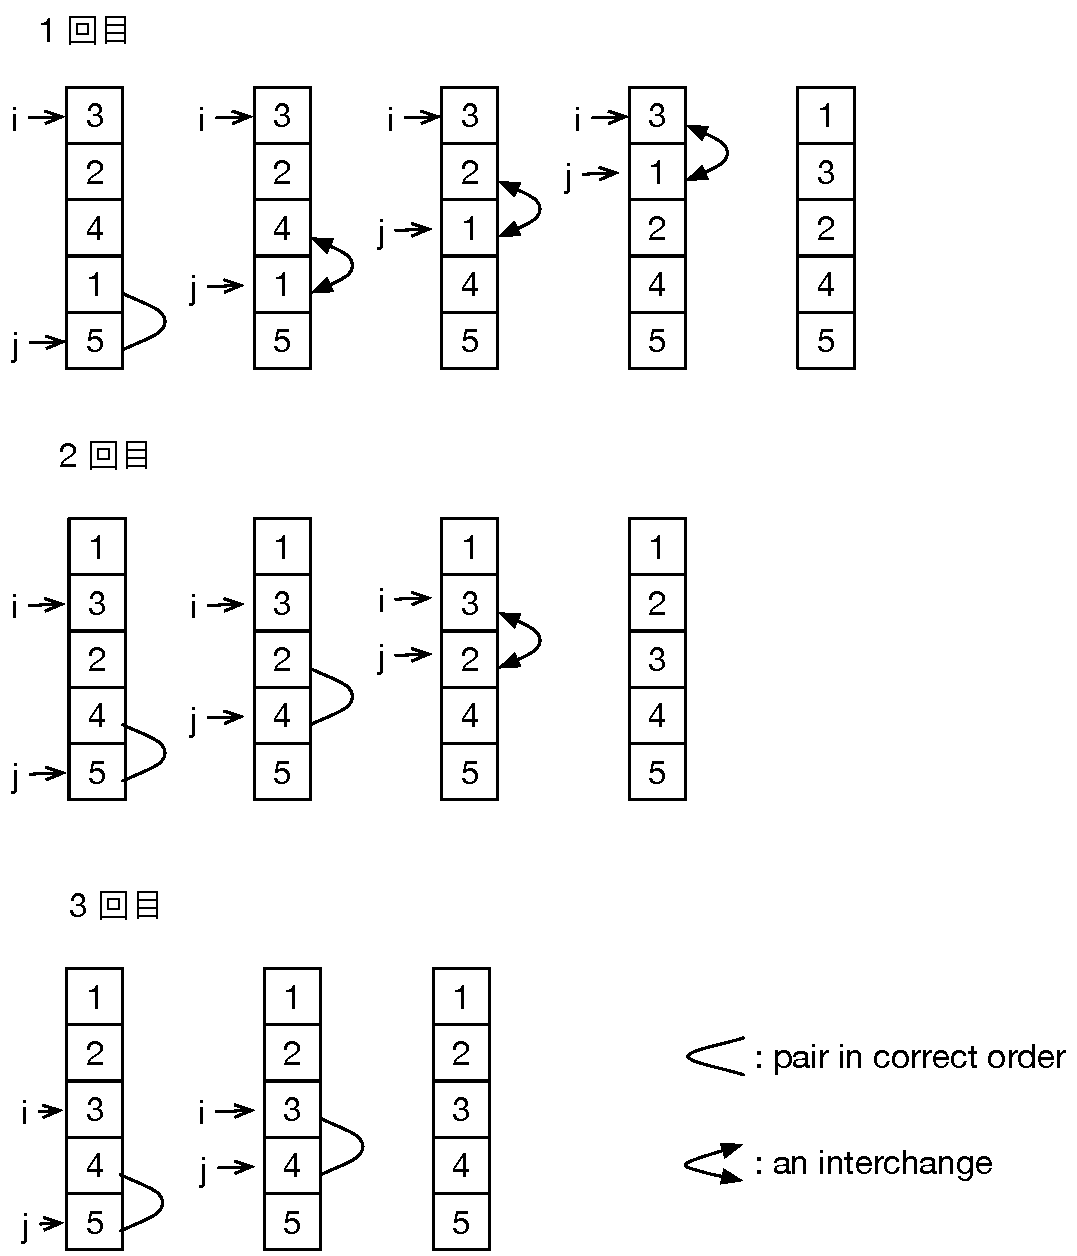
\includegraphics[scale=0.4]{./Figure/bubble_sort.pdf}
  \end{center}
\end{frame}
\begin{frame}[shrink]
\frametitle{Insertion Sort}
  \begin{center}
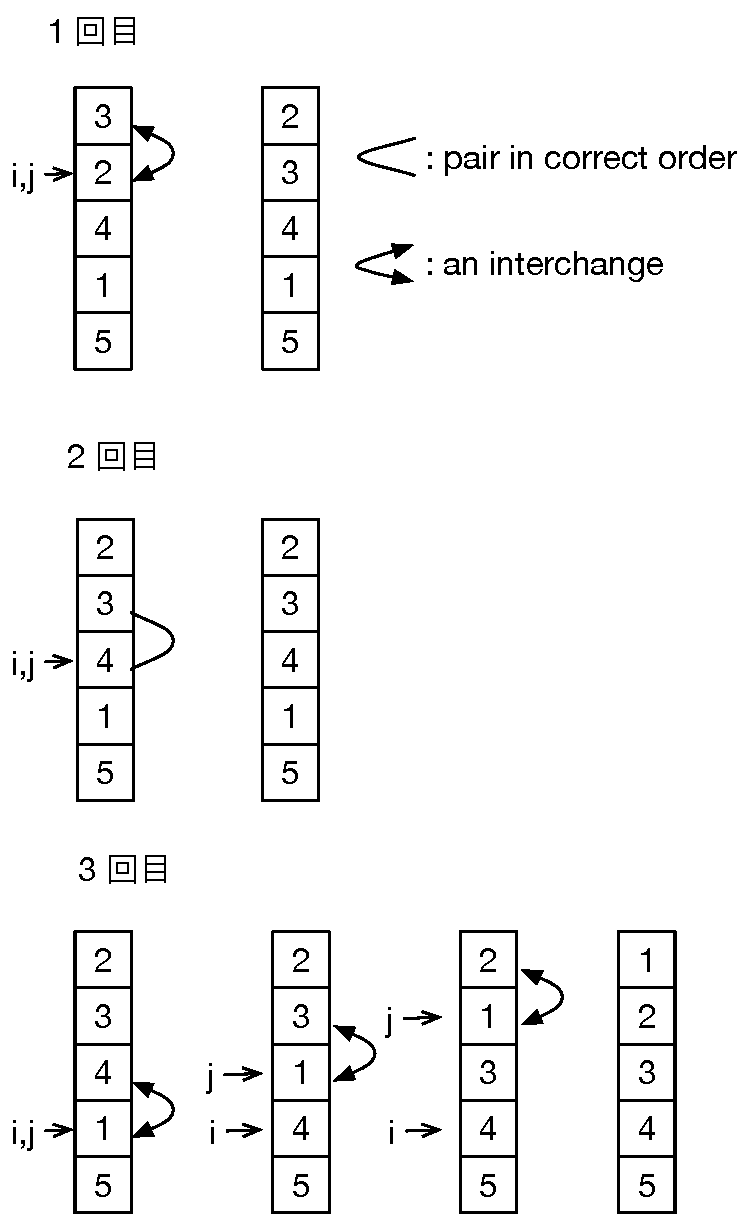
\includegraphics[scale=0.4]{./Figure/insertion_sort.pdf}
  \end{center}
\end{frame}
\begin{frame}[shrink]
\frametitle{Quiz 3}
\framesubtitle{Sort}
  \begin{block}{Quiz: Quick Sort}
\scriptsize
    \begin{itemize}
\item Input: 任意の長さの任意の整数の列
\item Output: 昇順に整列した列
\item sort-skeleton.py を加筆して quick sort を作成して実行時間を比較して見てください
\item 提出は sort.py としてソースコードだけ提出
\item ソースコードの先頭にコメント行で quick sort のオーダを入れておいてください (option)
    \end{itemize}
  \end{block}
  \begin{center}
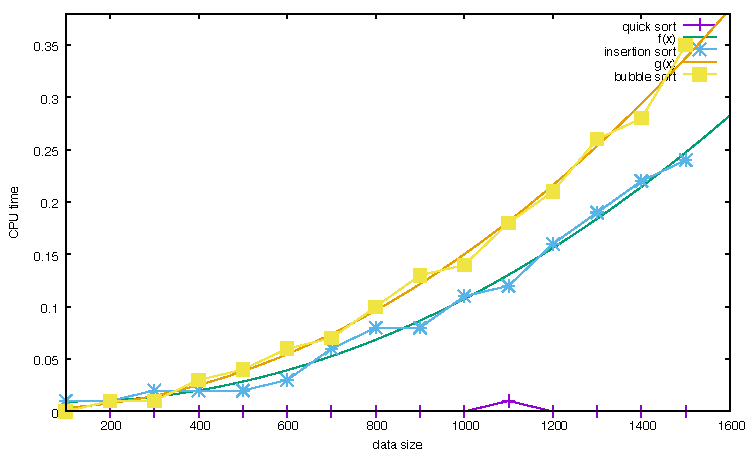
\includegraphics[scale=0.6]{./progs/sort.pdf}
  \end{center}
\end{frame}
\begin{frame}[shrink]
\frametitle{Quiz 3 の hint}
  \begin{itemize}
\scriptsize
\item Basic step: 異なる値がないときには終了
\item Recursive step:
    \begin{enumerate}
\scriptsize
\item 中間付近の値 pivot を選ぶ
\item pivot より小さい値を左側に,大きい値を右側に集める
\item 左側,右側でそれぞれソートする
    \end{enumerate}
  \end{itemize}
  \begin{center}
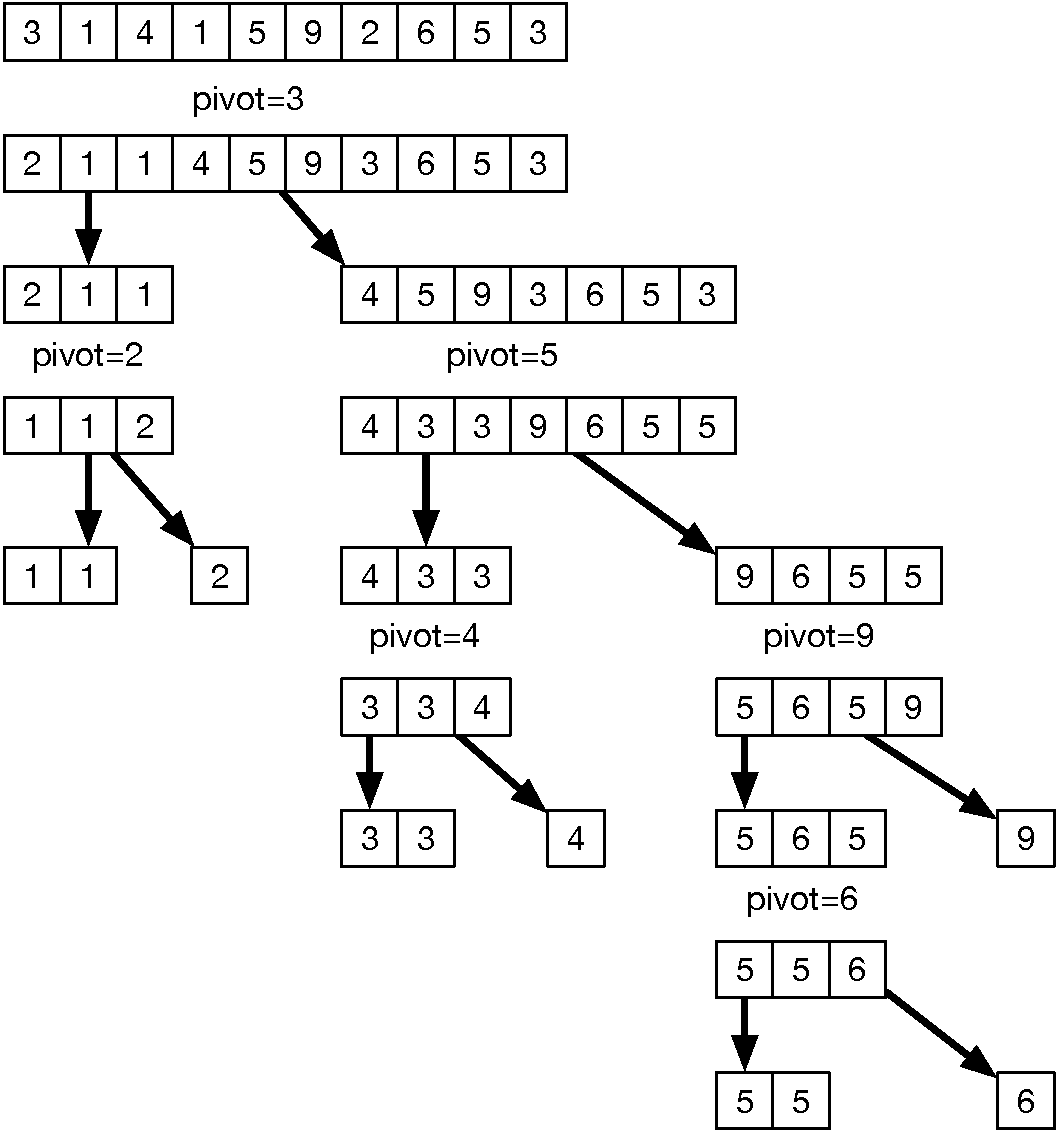
\includegraphics[scale=0.3]{./Figure/quick_sort.pdf}
  \end{center}
\end{frame}
\section{Search Alogorithms}
\begin{frame}
\frametitle{Option Quiz}
\framesubtitle{Search}
  \begin{itemize}
\item 余裕のある人は search algorithms のプログラムに挑戦してみてください
\item Linear search と binary search のプログラムを作成し実行時間を比べる
  \end{itemize}
\end{frame}
%%% Shortest Path Problem
%
%\section{最適解を求める問題}
\begin{frame}
\frametitle{最短経路問題}
  \begin{itemize}
\item カーナビや乗換案内や地図で所要時間の短い経路や旅費の安い経路を案内してくれるます
\item これはグラフ理論 (Graph Theory) と呼ばれる世界の最短経路問題に帰着できます
\item 与えられた条件で最適解を求めるという問題
  \end{itemize}
  \begin{block}{余裕のある人向け quiz}
    \begin{itemize}
\item 出発地と到着地がそれぞれ与えられたとしてコストが最も小さい経路を計算するプログラムを作成してください
\item $n$ 個の node を持つとして \(O(n^2)\) のオーダで計算できます
\item グラフの表現方法を変えると \(O(n\log n)\) にできます
    \end{itemize}
  \end{block}
\end{frame}
\begin{frame}
\frametitle{グラフ理論}
  \begin{itemize}
\item グラフとはあるデータ間の関係だけに注目したモデル
\item $N$ をノードの集合 (a set of nodes), $E$ をエッジの集合 (a set of edges) としてグラフ $G$ は \((N,E)\) の対である
\item 各ノードとエッジにはラベルが付けられていて,ラベルの集合を $L$ とする
  \end{itemize}
  \begin{center}
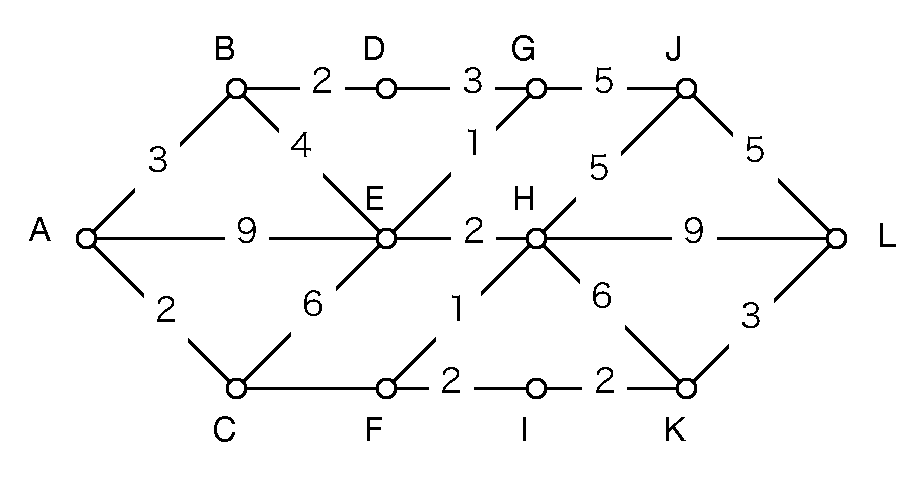
\includegraphics[scale=0.5]{./Figure/elementaryCS-2nd-figSPP.eps}
  \end{center}
\end{frame}
\begin{frame}
\frametitle{最短経路問題 (Shortest Pahts Problem)}
  \begin{itemize}
\item \(G=(N,E)\) で各エッジにコストでラベル付けし,
\item 任意の出発点が与えられたとして,他の地点に至る最小コストの経路を求める問題
  \end{itemize}
  \begin{columns}
    \begin{column}{0.3\textwidth}
      \begin{center}
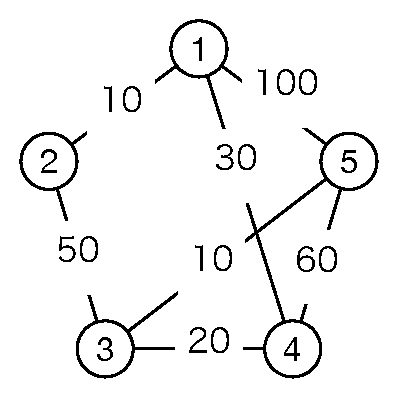
\includegraphics[scale=0.35]{./Figure/elementaryCS-2nd-figSPP-Sample.eps}
      \end{center}
    \end{column}
    \begin{column}{0.65\textwidth}
      \begin{center}
\footnotesize
        \begin{tabular}{cccccc}
S&w&D[2]&D[3]&D[4]&D[5]\\
\hline
\{1\}&\textendash&10&&30&100\\
\{1,2\}&2&10&60&30&100\\
\{1,2,4\}&4&10&50&30&90\\
\{1,2,4,3\}&3&10&50&30&60\\
\{1,2,4,3,5\}&5&10&50&30&60
        \end{tabular}
      \end{center}
    \end{column}
  \end{columns}
\end{frame}

\section{計算の複雑さのクラス}
\begin{frame}[shrink]
\frametitle{計算の複雑さのクラス}
  \begin{itemize}
\item 計算量をオーダであらわすことをみてきました
\item 計算量的に実行可能であるかという境界はどこにあるか,という疑問が出てくるのは自然なこと
\item ひとつは多項式境界 (polinomial bound) でこのクラスを P (Polynominal time) と表し,
\item もう一つを指数境界 (exponential bound) でこのクラスを NP (Non-deterministic Polynomial time) と表す.
    \begin{itemize}
\item このふたつは,決定性か非決定性かの違いや,
\item 解を得るのに全数探索しなければならないかどうかの違いとして見て取れる
    \end{itemize}
\item 有名な問題が \(\mbox{P}\neq\mbox{NP}\) かどうかという問題
  \end{itemize}
\end{frame}

%
%%% 実数
%
%\part{大きい数と小さい数の計算}
%\frame{
%  \frametitle{大きい数と小さい数の計算}
%\scriptsize
%  \tableofcontents[part=4]
%}
%\section{数の表現}
\begin{frame}[shrink]
\frametitle{繰り返しや再帰によるその他の計算}
  \begin{itemize}
\item 繰り返しや再帰は自然数 $n$ に対応する解を求めるような感じ
    \begin{itemize}
\item 数列は $n$ 番目の数を求める: \(\alpha\colon N\rightarrow N\)
\item ハノイの塔も $n$ 枚目の解を求める
    \end{itemize}
\item これを利用して関数の解を求める計算に利用する
\item たとえば非線形方程式 \(f(x)=0\) の実根を求める
\item \href{run:newton.command}{\beamerbutton{ニュートン法}}
    \begin{itemize}
\item \(\sqrt{a}\) を求めてみる
\item \(f(x)=x^2-a\) として \(f(x)=0\) となる $x$ を求める
\item \(k+1\) 番目の近似値 \(x_{k+1}\) を
      \begin{displaymath}
x_{k+1} = x_k-\frac{f(x_k)}{f'(x_k)} = \frac{1}{2}(x_k+\frac{a}{x_k})
      \end{displaymath}
で求める
\item \(x_{k+1}\) と \(x_k\) が十分近くなったら停止
    \end{itemize}
  \end{itemize}
\end{frame}
\subsection{非負整数の表現}
\begin{frame}[label=Top_Integer]
\frametitle{非負整数のコンピュータ内での表現}
  \begin{itemize}
\item 10 進数から 2 進数への変換
  \end{itemize}
  \begin{center}
   \begin{example}[10進$\Leftrightarrow$2進]
   \begin{columns}[t]
    \begin{column}{3cm}
\infer[\mbox{High}]{0}{\infer{2)1\cdots 1}{\infer{2)2\cdots 0}{\infer{2)4\cdots 0}{\infer[\mbox{Low}]{2)9\cdots 1}{2)19\cdots 1}}}}}
    \end{column}
    \begin{column}{3cm}
\infer{19}{\infer{1\times 2^4=16}{\infer{0\times 2^3=0}{\infer{0\times 2^2=0}{\infer{1\times 2^1=2}{1\times 2^0=1}}}}}
    \end{column}
   \end{columns}
   \end{example}
  \end{center}
\end{frame}
\subsection{負の数の表現}
\begin{frame}[shrink]
\frametitle{負の数の表現}
  \begin{itemize}
\item 負の数をあらわすには補数表現をもちいます
\item それでは 2 の補数(2's complement) を求めてみましょう
  \end{itemize}
  \begin{block}{2 の補数表現}
    \begin{enumerate}
\item 2 進表記において各ビットを反転する
\item それに 1 を足す
    \end{enumerate}
  \end{block}
  \begin{center}
    \begin{example}[-8$\sim$7 (2 進 4 桁) の 2 の補数表現]
\((1000)_{(2)}\Rightarrow(1001)_{(2)}\Rightarrow(1010)_{(2)}\Rightarrow (1011)_{(2)}\Rightarrow (1100)_{(2)}
\Rightarrow(1101)_{(2)}\Rightarrow(1110)_{(2)}\Rightarrow(1111)_{(2)}
\Rightarrow(0000)_{(2)}\Rightarrow(0001)_{(2)}\Rightarrow(0010)_{(2)}\Rightarrow(0011)_{(2)}
\Rightarrow(0100)_{(2)}\Rightarrow(0101)_{(2)}\Rightarrow(0110)_{(2)}\Rightarrow(0111)_{(2)}\)\\
      \begin{itemize}
\item Successor (1 足す) でつぎの数になるようになっている
\item 最上位ビットがサインビットになっている
\item circulation の実行
      \end{itemize}
    \end{example}
  \end{center}
\end{frame}
\subsection{計算機内の計算}
\begin{frame}[shrink]
\frametitle{計算機内の計算}
\framesubtitle{整数の減算}
  \begin{itemize}
\item 2 進 $n$ 桁の数 $a, b$ (\(A_k,B_k\in\{1,0\}\))
    \begin{itemize}
\item \(a\colon A_{n-1}A_{n-2}\cdots A_{1}A_{0}\)
\item \(b\colon B_{n-1}B_{n-2}\cdots B_{1}B_{0}\)
    \end{itemize}
\item \(a, b\) はそれぞれ
\[a=\sum_{k=0}^{n-1}2^{k}A_{k}\]
\[b=\sum_{k=0}^{n-1}2^{k}B_{k}\]
\item $b$ の各桁を反転させたものを \(\overline{B_{k}}\) として $b$ の補数 \(\overline{b}\) は
\[\overline{b}=\sum_{k=0}^{n-1}2^{k}\overline{B_{k}}=\sum_{k=0}^{n-1}2^{k}(1-B_{k})=(2^n-1)-b\]
  \end{itemize}
\end{frame}
\begin{frame}[shrink]
\frametitle{計算機内の計算\textemdash Cont.}
  \begin{itemize}
\item \(\overline{b}=(2^n-1)-b\) より
    \begin{eqnarray*}
a-b&\Rightarrow& a-((2^n-1)-\overline{b})\\
   &=&a+\overline{b}+1-2^n
    \end{eqnarray*}
\item 引き算は補数を足すことで表す
\item \(\overline{b}+1\) は 2 の補数
\item \(-2^n\) は最上位の桁上がりは無視
  \end{itemize}
  \begin{example}[引き算の例]
    \begin{itemize}
\item 4 桁の2進数と仮定して \(6-3\) と \(3-6\)
    \end{itemize}
    \begin{columns}[t]
      \begin{column}{3.5cm}
        \begin{tabular}{ccccc}
&0&1&1&0\\
$+$&1&1&0&1\\
\hline
&0&0&1&1\\
        \end{tabular}
      \end{column}
      \begin{column}{3.5cm}
        \begin{tabular}{ccccc}
&0&0&1&1\\
$+$&1&0&1&0\\
\hline
&1&1&0&1\\
        \end{tabular}
      \end{column}
    \end{columns}
  \end{example}
\end{frame}

%\subsection{実数の表現}
\begin{frame}[shrink]
\frametitle{実数の表現}
\framesubtitle{浮動小数 (floating point number)}
  \begin{itemize}
\item 浮動小数 \(ab^{e}\)
    \begin{itemize}
\item $a$ は仮数 (significand or coefficient) ,$b$ は底 (base),$e$ は指数 (exponent) と呼ぶ
    \end{itemize}
\item \(\frac{1}{b}\leq|a|<1\) のとき正規浮動小数 (normalized floating point number) と云う
\item 上のような変換を正規化(normalizaiton) と云う
\item 符号,指数,仮数で一意に決定できます
  \end{itemize}
  \begin{example}[正規浮動小数]
   \begin{math}
    \begin{array}{rcl}
1.234 &\Rightarrow& +0.1234\times 10^1\\
-12.34 &\Rightarrow& -0.1234\times 10^2\\
0.01234 &\Rightarrow& +0.1234\times 10^{-2}\\
    \end{array}
   \end{math}
  \end{example}
\end{frame}
\begin{frame}
\frametitle{実数の 2 進表記}
  \begin{itemize}
\item 実数も 2 進表記に変換した上で正規化します
\item 13.6875$_{(10)}$ を2進数へ変換してみます
  \end{itemize}
  \begin{center}
   \begin{example}[10進実数 13.6875$_{(10)}$ を2進数へ]
     \begin{columns}[t]
       \begin{column}{4.5cm}
\infer[High]{0}{\infer{2)1\cdots 1}{\infer{2)3\cdots 1}{\infer[Low]{2)6\cdots 0}{2)13\cdots 1}}}}
         \begin{itemize}
\item 13$_{(10)}$ は 1101$_{(2)}$
         \end{itemize}
       \end{column}
     \begin{column}{4.5cm}
\infer[Low]{.5\times 2=1.00}{\infer{.75\times 2=1.50}{\infer[High]{.375\times 2=0.75}{.6875\times 2=1.375}}}
     \begin{itemize}
\item .6875$_{(10)}$ は .1011$_{(2)}$
     \end{itemize}
      \end{column}
     \end{columns}
     \begin{itemize}
\item ゆえに, 13.6875$_{(10)}$ は 1101.1011$_{(2)}$ となる 
     \end{itemize}
   \end{example}
  \end{center}
\end{frame}
\begin{frame}
\frametitle{実数の 2 進表記 - Cont.}
  \begin{itemize}
\item 得られた 2 進数を正規化します
\item 最上位ビットが 1 になるようにします (注意: 正規化の定義と違っているので注意)
  \end{itemize}
  \begin{center}
    \begin{example}[1101.1011$_{(2)}$ を正規化]
1101.1011$_{(2)}$ \(\Rightarrow\) 0.11011011\(\times 2^4\)
      \begin{itemize}
\item 符号: +
\item 指数: 4
\item 仮数: 0.11011011
      \end{itemize}
    \end{example}
  \end{center}
\end{frame}
\begin{frame}[shrink]
\frametitle{実数の 2 進表記 - Cont.}
  \begin{itemize}
\item 符号,指数,仮数が正規化によって決まります
\item これを 32 ビットで表す
\item 右に小数点を一つ移動
\item 最上位ビットは必ず 1 になるので省略
\item 規格 \href{http://ieeexplore.ieee.org/xpl/mostRecentIssue.jsp?punumber=2355}{\beamerbutton{IEEE 754}} はもうひと段階
  \end{itemize}
  \begin{center}
    \begin{example}[指数部,仮数部]
      \begin{itemize}
\item 1.1011011\(\times 2^3\) の符号,指数,仮数は以下のとおり
        \begin{itemize}
\item 符号 (sign): +
\item 指数 (exponent): 3
\item 仮数 (significand): 1.1011011
        \end{itemize}
      \end{itemize}
    \end{example}
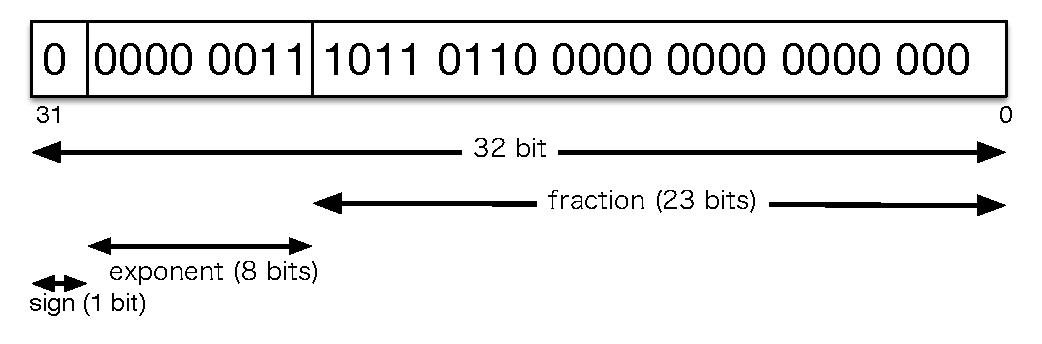
\includegraphics[scale=.4]{./Figure/elementaryCS-figFloatingPointFormat.eps}
  \end{center}
\end{frame}
\begin{frame}
\frametitle{宿題 3: 浮動小数}
  \begin{itemize}
\item 実数の浮動小数表現をやってみてください
  \end{itemize}
  \begin{block}{宿題 3}
    \begin{itemize}
\item 35.75 を浮動小数で表現してみてください
\item T2Schola に小テストがあるのでそれに答えてください
    \end{itemize}
  \end{block}
\end{frame}
\begin{frame}
\frametitle{宿題 3: 回答}
  \begin{itemize}
\item 2 進へ変換: 100011.11
\item 正規化: 1.0001111$\times 2^5$
\item 32 bit 形式に: {\scriptsize 0 0000 0101 0001 1110 0000 0000 0000 000}
    \begin{itemize}
\item 1. は省略
    \end{itemize}
\item 規格\href{http://ieeexplore.ieee.org/xpl/mostRecentIssue.jsp?punumber=2355}{\beamerbutton{IEEE 754}}では下駄 (bais) をはかせるので\(5+127=132\Rightarrow\) 1000 0100
\item 32 bit 形式に: {\scriptsize 0 1000 0100 0001 1110 0000 0000 0000 000}
  \end{itemize}
\end{frame}
\subsection{浮動小数の算術演算}
\begin{frame}[shrink,fragile]
\frametitle{浮動小数演算の変な現象 1}
  \begin{itemize}
\item roundoff.py を実行してみます
\item 結果が予測と少し違うことになります
\item \(0.6_{(10)}\) は \((0.1001\ldots)_{(2)}\), \(0.4_{(10)}\) は \((0.0110\ldots)_{(2)}\), \(0.2_{(10)}\) は \((0.0011\ldots)_{(2)}\) となります
  \end{itemize}
  \begin{lstlisting}[caption={roundoff.py},label=lst:roundoff]
if (float(0.6)-float(0.4)==float(0.2)):
   print("is equal")
else:
   print("not equal")
  \end{lstlisting}
\end{frame}
\begin{frame}[shrink,fragile]
\frametitle{浮動小数演算の変な現象 2}
  \begin{itemize}
\item machine\_epsilon.py を実行してみます
\item 結果が予測と少し違うことになります
\item この原因についてみていきます
  \end{itemize}
  \begin{lstlisting}[caption={machine\_epsilon.py},label=lst:epsilon]
# Machine epsilon
import sys

epsilon, old, prod =1.0, 0.0, 0.0
cnt=0
while (prod!=1.0):
  print(epsilon)
  old = epsilon
  cnt=cnt+1
  epsilon=epsilon/2.0
  prod=epsilon+1.0
print("Calculated machine epsilon:",old)
print("System information in Python:",sys.float_info.epsilon)
  \end{lstlisting}
\end{frame}
\begin{frame}[shrink]
\frametitle{浮動小数数の算術演算}
  \begin{itemize}
\item 正規化した 2 つの浮動小数 \(X, Y\) を \(X=F_x\times 10^{e_x}, Y=F_y\times 10^{e_y}\) とする
\item 乗算: \(XY=(F_x\times 10^{e_x})(F_y\times 10^{e_y})=F_xF_y\times 10^{e_x+e_y}\)
\item 除算: \(\frac{X}{Y}=\frac{(F_x\times 10^{e_x})}{(F_y\times 10^{e_y})}=\frac{F_x}{F_y}\times 10^{e_x-e_y}\)
\item 加算\(\cdot\)減算: \(X\pm Y=(F_x\times 10^{e_x})\pm(F_y\times 10^{e_y})=(F_x\pm F_y\cdot 10^{e_y-e_x})\times 10^{e_x}\)
    \begin{itemize}
\item ただし,\(e_x\geq e_y\)
\item \(F_y\cdot 10^{e_y-e_x}\) は指数を大きい方に揃えたときの $Y$ の仮数
    \end{itemize}
\item 演算結果も正規化するので指数は調整が必要
  \end{itemize}
  \begin{example}[算術演算の例]
    \begin{columns}[t]
      \begin{column}{4.5cm}
        \begin{math}
          \begin{array}{cll}
&0.2184&\times 10^2\\
\times&0.2512&\times 10^2\\
\hline
&0.07998208&\times 10^4\\
=&0.7998208&\times 10^3\\
          \end{array}
        \end{math}
      \end{column}
      \begin{column}{4.5cm}
        \begin{math}
          \begin{array}{cll}
&0.2844&\times 10^3\\
+&0.4162&\times 10^1\\
\hline
&0.288562&\times 10^3\\
          \end{array}
        \end{math}
      \end{column}
    \end{columns}
  \end{example}
\end{frame}
%\begin{frame}
%\frametitle{算術演算の誤差}
%  \begin{itemize}
%\item 4 桁までしか記憶できないと仮定
%\item \(0.2844\cdot 10^3+0.4162\cdot 10^1=0.288562\cdot 10^3=(0.2885+0.000062)\cdot 10^3=0.2885\cdot 10^3+0.6200\cdot 10^{-1}\)
%\item \(0.288562\)が真の値となるが \(0.2885\) までしか記憶できないので
%\item \(0.6200\cdot 10^{-1}(=0.000062\cdot 10^3)\) について調整する必要がある
%  \end{itemize}
%  \begin{example}[\(0.2844\cdot 10^3+0.4162\cdot 10^1\)]
%    \begin{columns}[t]
%      \begin{column}{4.5cm}
%        \begin{math}
%          \begin{array}{cll}
%&0.2844&\times 10^3\\
%+&0.4162&\times 10^1\\
%\hline
%&0.288562&\times 10^3\\
%          \end{array}
%        \end{math}
%      \end{column}
%      \begin{column}{4.5cm}
%        \begin{math}
%          \begin{array}{cll}
%&0.2844&\times 10^3\\
%+&0.004162&\times 10^3\\
%\hline
%&0.288562&\times 10^3\\
%          \end{array}
%        \end{math}
%      \end{column}
%    \end{columns}
%  \end{example}
%\end{frame}
\section{誤差のおはなし}
\subsection{丸め誤差 (roundoff error)}
\begin{frame}[shrink]
\frametitle{誤差とは}
  \begin{itemize}
\item コンピュータの中では実数は有限個の 0 と 1 の組み合わせ(浮動小数)で表しています
\item なので,本来あるべき真値を適当な浮動小数で近似している
\item 近似値-真値 を誤差という
  \end{itemize}
\end{frame}
\begin{frame}[shrink]
\frametitle{丸め誤差 (roundoff error)}
  \begin{itemize}
\item 表現可能な範囲に丸めることを丸め誤差という(\lstref{lst:roundoff}参照)
\item 演算結果も丸める
\item $Z$ を演算結果とする
\item $d$ 桁だけ記憶できるとして,先頭の $d$ 桁を $F$,残りを $f$ とすると,\(Z=F\cdot 10^{e_z}+f\cdot 10^{e_z-d}\)
\item $f$ の値で四捨五入することにして
    \begin{displaymath}
      \begin{array}{ll}
|f|<0.5 \mbox{のとき} & |Z|=|F|\cdot 10^{e_z-d}\\
|f|\geq 0.5 \mbox{のとき} & |Z|=|F|\cdot 10^{e_z-d}+\cdot 10^{e_z-d}
      \end{array}
    \end{displaymath}
\item 丸め誤差 $\epsilon_z$ とすれば
    \begin{displaymath}
      \begin{array}{ll}
|f|<0.5 \mbox{のとき} & |\epsilon_z|=|f|\cdot 10^{e_z-d}\\
|f|\geq 0.5 \mbox{のとき} & |\epsilon_z|=|1-f|\cdot 10^{e_z-d}
      \end{array}
    \end{displaymath}
  \end{itemize}
  \begin{example}[\(0.2844\cdot 10^3+0.4162\cdot 10^1\)]
    \begin{itemize}
\item \(0.2844\cdot 10^3+0.4162\cdot 10^1=0.2885\cdot 10^3+0.6200\cdot 10^{-1}\)
\item \(|Z|=0.2885\cdot 10^3+10^{3-4}=0.2886\cdot 10^3\)
\item \(|\epsilon_z|=|1-0.6200|\cdot 10^{3-4}=0.48\cdot 10^{-1}\)
    \end{itemize}
  \end{example}
\end{frame}
%\begin{frame}
%\frametitle{相対誤差 (relative error)}
%  \begin{itemize}
%\item 計算のコストだけでなくときには計算精度も重要になる
%\item 真の値 $x^t$,観測した値 $x$ として誤差 \(\epsilon_x=x^t-x\)
%\item \(|\epsilon_x|=|x^t-x|\) を絶対誤差という
%\item 相対誤差 \(r_x=\frac{\epsilon_{x}}{x}=\frac{x^t-x}{x}\) で精度を測る
%  \end{itemize}
%  \begin{example}[相対誤差の例]
%    \begin{itemize}
%\item \(x_t=9, x=10\) と \(y_t=999, y=1000\) の場合を考える
%\item $x$ と $y$ の誤差はどちらも \(-1\)
%\item $x$ と $y$ の相対誤差はそれぞれ \(r_x=\frac{-1}{10}, r_y=\frac{-1}{1000}\)
%    \end{itemize}
%  \end{example}
%\end{frame}
%\subsection{誤差の伝搬 (propagation of errors)}
%\begin{frame}
%\frametitle{誤差の伝搬 (propagation of errors)}
%  \begin{itemize}
%\item 誤差は計算中伝播して計算結果を不正確にしてしまう
%\item 算術式中の誤差がどう蓄積されていくかをみる
%\item ある数 $x, y$ としてそれぞれが誤差 \(\epsilon_x, \epsilon_y\) を持つとする
%\item このときの演算 \(x\oplus y\) の誤差 \(\epsilon_{x\oplus y}\) は
%    \begin{displaymath}
%\epsilon_{x\oplus y}=(x^t\oplus y^t)-(x\oplus y)
%    \end{displaymath}
%\item \(x^t\oplus y^t\) は真の演算結果で, \(x\oplus y\) は実際の結果
%\item 先の誤差の定義からこれが導ける
%  \end{itemize}
%\end{frame}
%\begin{frame}[shrink]
%\frametitle{誤差公式}
%  \begin{itemize}
%\item 各演算についてつぎの関係が成り立つ
%  \end{itemize}
%  \begin{theorem}[誤差公式]
%    \begin{math}
%      \begin{array}{lclclclcl}
%\scriptsize
%\epsilon_{x+y}&=&(x^t+y^t)-(x+y)&=&(x^t-x)+(y^t-y)&=&\epsilon_x+\epsilon_y\\
%\epsilon_{x-y}&=&(x^t-y^t)-(x-y)&=&(x^t-x)-(y^t-y)&=&\epsilon_x-\epsilon_y\\
%      \end{array}
%    \end{math}
%    \begin{math}
%      \begin{array}{lclclclcl}
%\epsilon_{xy}&=&(x^ty^t)-(xy)&=&(x+\epsilon_x)(y+\epsilon_y)-(xy)&=&\epsilon_x y+\epsilon_y x\\
%      \end{array}
%    \end{math}
%    \begin{math}
%      \begin{array}{lclclclcl}
%\epsilon_{\frac{x}{y}}&=&\frac{x^t}{y^t}-\frac{x}{y}&=&\frac{x^ty-y^tx}{y^ty}&=&\frac{(x+\epsilon_x)y-(y+\epsilon_y)x}{(y+\epsilon_y)y}\\
%&=&\frac{xy+\epsilon_xy-xy+x\epsilon_y}{y^2(1+\frac{\epsilon_y}{y})}&=&\frac{\epsilon_xy-\epsilon_yx}{y^2}\\
%      \end{array}
%    \end{math}
%    \begin{itemize}
%\item \(\epsilon_x\epsilon_y\) は十分小さいとして無視
%\item \(|\frac{\epsilon_y}{y}|\) は \(|\frac{\epsilon_y}{y}|\ll 1\) のとき無視
%\item これに各演算の丸め誤差 \(\alpha\) を加えたて誤差公式とする
%      \begin{itemize}
%\item たとえば 4 桁までしか記憶できないのであれば演算結果も 4 桁に丸められる
%      \end{itemize}
%    \end{itemize}
%  \end{theorem}
%\end{frame}
%\begin{frame}[shrink]
%\frametitle{相対誤差公式}
%  \begin{itemize}
%\item 相対誤差公式を導く
%\item 先の相対誤差の定義より
%    \begin{displaymath}
%r_{x\oplus y}=\frac{\epsilon_{x\oplus y}}{x\oplus y}
%    \end{displaymath}
%\item とすれば誤差公式よりつぎの相対誤差公式をえる
%  \end{itemize}
%  \begin{theorem}[相対誤差公式]
%    \begin{math}
%      \begin{array}{rclcl}
%r_{x+y}&=&\frac{\epsilon_x+\epsilon_y}{x+y}+\alpha&=&r_x\frac{x}{x+y}+r_y\frac{y}{x+y}+\alpha\\
%r_{x-y}&=&\frac{\epsilon_x-\epsilon_y}{x-y}+\alpha&=&r_x\frac{x}{x-y}+r_y\frac{-y}{x-y}+\alpha\\
%r_{xy}&=&\frac{\epsilon_x y+\epsilon_y x}{xy}+\alpha&=&r_x\ 1+r_y\ 1+\alpha\\
%r_{xy}&=&\frac{\frac{\epsilon_x y-\epsilon_y x}{y^2}}{\frac{x}{y}}+\alpha&=&r_x\ 1+r_y\ (-1)+\alpha
%      \end{array}
%    \end{math}
%  \end{theorem}
%\end{frame}
%\begin{frame}[shrink]
%\frametitle{誤差伝播の解析}
%  \begin{itemize}
%\item 相対誤差公式を使って誤差伝播の解析を行う
%  \end{itemize}
%  \begin{example}[和における誤差伝播]
%    \begin{itemize}
%\item \(r_0, r_1, r_2, r_3\) を実数 \(a_0,a_1,a_2,a_3\) の相対誤差とする
%\item \(S=(((a_0+a_1)+a_2)+a_3)\) の相対誤差を求める
%    \end{itemize}
%  \end{example}
%\end{frame}
\subsection{情報落ち誤差}
\begin{frame}[shrink]
\frametitle{情報落ち誤差(loss of trailing digits)}
  \begin{itemize}
\item 絶対値が大きく異なる 2 つの数の加減算では小さい数が無視されることがある
\item \lstref{lst:epsilon} で見たような場合
  \end{itemize}
\end{frame}
\subsection{打ち切り誤差 (truncation error)}
\begin{frame}[shrink]\label{sl:back}
\frametitle{打ち切り誤差 (truncation error)}
  \begin{itemize}
\item コンピュータでは無限に繰り返して値をもとめることはできない
\item 有限回の計算で値を計算し,それを求める値の近似値としてもちいる
\item このときの誤差を打切り誤差という
  \end{itemize}
  \begin{example}[\(\sin(x)\)のマクローリン展開]
    \begin{itemize}
\item \(sin(x)=x-\frac{x^3}{3!}+\frac{x^5}{5!}-\frac{x^7}{7!}+\cdots+(-1)^{n}\frac{x^{2n+1}}{(2n+1)!}+\cdots\)
\item gnuplot で試してみてください
    \end{itemize}
  \end{example}
  \begin{example}[平方根の計算]
    \begin{itemize}
%\item \href{run:newton.command}{\beamerbutton{ニュートン法}}
\item newton.py を参照\hyperlink{newton-is_enough-rec}{\beamerbutton{プログラム例}}
\item \(\sqrt{a}\) を求めてみる
\item \(f(x)=x^2-a\) として \(f(x)=0\) となる $x$ を求める
\item \(k+1\) 番目の近似値 \(x_{k+1}\) を
      \begin{displaymath}
x_{k+1} = x_k-\frac{f(x_k)}{f'(x_k)} = \frac{1}{2}(x_k+\frac{a}{x_k})
      \end{displaymath}
    \end{itemize}
  \end{example}
\end{frame}
%\section{まとめ}
%\begin{frame}[shrink,fragile]
%\frametitle{数値計算}
%  \begin{itemize}
%\item ここで取り上げたおはなしは数値計算(計算機科学の一分野)のなかの計算誤差をとりあげたもの
%\item シミュレーションなどではある関数の実際の数値を必要とする場合がある
%    \begin{itemize}
%\item 例えば,方程式 \(f(x)=0\) の $x$ を数値的に求める
%    \end{itemize}
%\item 数値計算の手順
%    \begin{itemize}
%\item 最初に適当な 1 次近似 \(x_0\) を選んで,
%\item より良い近似を求め,
%\item 適当な収束条件を満たすまで繰り返す (マシンイプシロンは収束条件の重要な指標)
%    \end{itemize}
%\item \(f\) は複雑なので数値的な解を求めるいろいろな算法を考察
%  \end{itemize}
%\end{frame}


\end{document}
